%\VignetteIndexEntry{Exploring diallelic genetic markers: the \pkg{HardyWeinberg} package}
\documentclass[nojss]{jss}
%\documentclass[article]{jss}
\usepackage[cp1252]{inputenc}
\usepackage{amsmath, amsfonts}
\usepackage{float,amssymb}
%\usepackage{hyperref}
\usepackage{latexsym}
\usepackage{wasysym}

\shortcites{Purcell}


%%%%%%%%%%%%%%%%%%%%%%%%%%%%%%
%% declarations for jss.cls %%%%%%%%%%%%%%%%%%%%%%%%%%%%%%%%%%%%%%%%%%
%%%%%%%%%%%%%%%%%%%%%%%%%%%%%%


%% almost as usual
\author{Jan Graffelman\\Universitat Polit\`ecnica de Catalunya\\version 1.6.3\\ \today}
\title{Exploring Diallelic Genetic Markers: The \pkg{HardyWeinberg} Package}

%% for pretty printing and a nice hypersummary also set:
\Plainauthor{Jan Graffelman} %% comma-separated
\Plaintitle{Exploring Equilibrium for Diallelic Genetic Markers: The \pkg{HardyWeinberg} Package} %% without formatting
\Shorttitle{HardyWeinberg Equilibrium in \proglang{R}} %% a short title (if necessary)

%% an abstract and keywords
\Abstract{
  Testing genetic markers for Hardy-Weinberg equilibrium is an
  important issue in genetic association studies. The
  \pkg{HardyWeinberg} package offers the classical autosomal tests for
  equilibrium, functions for power computation and for the simulation
  of marker data under equilibrium and disequilibrium. Recently, specific 
  frequentist and Bayesian tests for X-chromosomal markers have been developed and included in the package. Functions 
for testing equilibrium in the presence of missing data by using multiple
imputation are provided. The package
  also supplies various graphical tools such as ternary plots with
  acceptance regions, log-ratio plots and Q-Q plots for exploring the
  equilibrium status of a large set of diallelic markers. Classical
  tests for equilibrium and graphical representations for diallelic
  marker data are reviewed. Several data sets illustrate the use of
  the package.
  
}
\Keywords{ternary plot, Q-Q plot, chi-square test, exact test, permutation test, power, log-ratio}
\Plainkeywords{ternary plot, Q-Q plot, chi-square test, exact test, permutation test, power, log-ratio} %% without formatting
%% at least one keyword must be supplied

%% publication information
%% NOTE: Typically, this can be left commented and will be filled out by the technical editor
%% \Volume{13}
%% \Issue{9}
%% \Month{September}
%% \Year{2004}
%% \Submitdate{2004-09-29}
%% \Acceptdate{2004-09-29}

%% The address of (at least) one author should be given
%% in the following format:
\Address{
  Jan Graffelman\\
  Department of Statistics and Operations Research\\
  Universitat Polit\`ecnica de Catalunya\\
  Barcelona, Spain\\
  E-mail: \email{jan.graffelman@upc.edu}\\
  URL: \url{http://www-eio.upc.es/~jan/}
}
%% It is also possible to add a telephone and fax number
%% before the e-mail in the following format:
%% Telephone: +43/1/31336-5053
%% Fax: +43/1/31336-734

%% for those who use Sweave please include the following line (with % symbols):
%% need no \usepackage{Sweave.sty}

%% end of declarations %%%%%%%%%%%%%%%%%%%%%%%%%%%%%%%%%%%%%%%%%%%%%%%


\begin{document}

\newcommand{\bx}{\ensuremath{\mathbf x}}
\newcommand{\pval}{$p$~value}
\newcommand{\pvals}{$p$~values}

\newcommand{\norm}[1]{\parallel\! #1 \!\parallel}
\newcommand{\deter}[1]{\mid\! #1 \!\mid}
\newcommand{\diag}[1]{\mbox{diag}(#1)}
\newcommand{\inv}[1]{{(#1)}^{-1}}
\newcommand{\invnp}[1]{{#1}^{-1}}
\newcommand{\chisq}{$\chi^2$}
\newcommand{\half}{\ensuremath{\frac{1}{2}}}
\newcommand{\abs}[1]{{|#1|}}
\newcommand{\etal}{{\it et al.}}
\newcommand{\sumn}{\sum_{i=1}^n}
\newcommand{\summ}{\sum_{i=1}^m}
\newcommand{\sumk}{\sum_{k=1}^n}
\newcommand{\sumxinf}{\sum_{x=1}^\infty}
\newcommand{\sumyinf}{\sum_{y=1}^\infty}
\newcommand{\Pro}[1]{P \left( #1 \right)}
\newcommand{\recip}[1]{\frac{1}{ #1 }}
\newcommand{\lne}[1]{\ln \left( #1 \right)}
\newcommand{\naa}{\ensuremath{n_{AA}}}
\newcommand{\nab}{\ensuremath{n_{AB}}}
\newcommand{\nbb}{\ensuremath{n_{BB}}}
\newcommand{\na}{\ensuremath{n_{A}}}
\newcommand{\nb}{\ensuremath{n_{B}}}
\newcommand{\eaa}{\ensuremath{e_{AA}}}
\newcommand{\eab}{\ensuremath{e_{AB}}}
\newcommand{\ebb}{\ensuremath{e_{BB}}}
\newcommand{\faa}{\ensuremath{f_{AA}}}
\newcommand{\fab}{\ensuremath{f_{AB}}}
\newcommand{\fbb}{\ensuremath{f_{BB}}}
\newcommand{\hfaa}{\ensuremath{\hat{f}_{AA}}}
\newcommand{\hfab}{\ensuremath{\hat{f}_{AB}}}
\newcommand{\hfbb}{\ensuremath{\hat{f}_{BB}}}
\newcommand{\faai}{\ensuremath{f_{AA_i}}}
\newcommand{\fabi}{\ensuremath{f_{AB_i}}}
\newcommand{\fbbi}{\ensuremath{f_{BB_i}}}
\newcommand{\naai}{\ensuremath{n_{AA_i}}}
\newcommand{\nabi}{\ensuremath{n_{AB_i}}}
\newcommand{\nbbi}{\ensuremath{n_{BB_i}}}
\newcommand{\midp}{mid}
\newcommand{\dos}{DOST}
\newcommand{\sel}{SELOME}
\newcommand\Real{ {\mathbb{R}} }        %real numbers/space
\newcommand{\gm}{ {\mathrm{g_m}} }      %geometric mean
\newcommand{\mbf}{ \mathbf }            %boldface for vectors and matrices
\newcommand{\mbfg}{ \boldsymbol }       %boldface for greek and number vectors/matrices
\newcommand{\clr}{ \mathrm{clr} }       % clr-transformation
\newcommand{\alr}{ \mathrm{alr} }       % alr-transformation
\newcommand{\ilr}{ \mathrm{ilr} }       % ilr-transformation

\section{Introduction}

The \pkg{HardyWeinberg} package~\citep{Graffel26} consists of a set of
tools for analyzing diallelic genetic markers in the \proglang{R}
environment~\citep{RRR}, and is particularly focused on the graphical
representation of their (dis)equilibrium condition in various ways.
The package is mainly aimed at researchers working in the fields of
genetics, statistics, epidemiology, bio-informatics and bio-statistics
and is available from the Comprehensive \proglang{R} Archive Network
(CRAN) at \url{http://CRAN.R-project.org/package=HardyWeinberg}.
This paper describes the state of the art of version 1.6.0 of the package. 
If you appreciate this software and wish to cite it, please cite the
corresponding paper in the {\it Journal of Statistical 
Software}~\citep{Graffel26}. 
The structure of this paper is as follows. In
Section~\ref{sec:hardyweinberg} we briefly introduce Hardy-Weinberg
equilibrium. Section~\ref{sec:tests} reviews the classical statistical
tests and power computation for Hardy-Weinberg
equilibrium. Section~\ref{sec:xchrom} briefly presents the X-chromosomal tests
for equilibrium. Section~\ref{sec:graphics} treats graphical
representations of Hardy-Weinberg equilibrium for sets of
markers. Section~\ref{sec:session} is an example session showing how
to analyze genetic markers with the functions of the package. Finally,
a discussion (Section~\ref{sec:others}) with some comments on related
packages completes the paper.


\section{Hardy-Weinberg equilibrium}
\label{sec:hardyweinberg}

A diallelic genetic marker with alleles {\sc a} and {\sc b} with
respective frequencies $p$ and $q$ ($p + q = 1$) is said to be in
Hardy-Weinberg equilibrium if the relative genotype frequencies \faa,
\fab\ and \fbb\ are given by $p^2$, $2pq$ and $q^2$ respectively. This
law, independently formulated by~\citet{Hardy} and~\citet{Weinberg},
is a fundamental principle of modern genetics~\citep{Crow}. The term
``Hardy-Weinberg equilibrium'' was proposed by~\citet{Stern}. The law
is easily extended to a system with multiple alleles $A_1, \ldots A_k$
with frequencies $p_1, \ldots, p_k$, giving genotype frequencies
$p_i^2$ for homozygotes and $2p_ip_j$ for heterozygotes. An
alternative formulation of the law for the diallelic case is obtained
by squaring the heterozygote frequency:
\begin{equation}
\fab^2 = 4 \faa \fbb.
\label{eq:hwe}
\end{equation}

Hardy-Weinberg equilibrium (HWE) is achieved in one generation of
random mating. In the absence of disturbing forces (migration,
mutation, selection, among other possibilities) the law predicts that
genotype and allele frequencies will remain in their equilibrium state
over the generations. We refer to genetic textbooks~\citep{Crow,Hartl}
for a more detailed treatment of the long list of assumptions that
underlie HWE. The law plays an important role in the context of
genetic association studies for various reasons. Disequilibrium may be
the result of genotyping error, most typically the confusion of
heterozygotes and homozygotes. Tests for HWE may thus help to detect
(gross) genotyping error. On the other hand, disequilibrium among
cases in a case-control study may be indicative of disease
association. Thus, tests for HWE may also provide clues in
marker-disease association studies.
\section{Classical autosomal tests for Hardy-Weinberg equilibrium}
\label{sec:tests}

There are several statistical tests available for investigating
whether a genetic marker can be considered to be in equilibrium or
not. The classical chi-square test for goodness-of-fit has been the
most popular test for HWE for decades, though nowadays exact
procedures are more and more often employed. A likelihood ratio test
is also available. A description of the different tests is given
by~\citet[Chapter 3]{Weir}. Bayesian inference for
HWE~\citep{Lindley,Ayres,Shoemaker,Wakefield,Consonni} is not
considered here. In the following sections we summarize the chi-square
test~(Section~\ref{subsec:chisquare}), the likelihood ratio
test~(Section~\ref{subsec:likelihood}), the exact test~(Section
\ref{subsec:exact}) and the permutation test~(\ref{subsec:permutation}), and also describe the computation of power for
HWE tests~(Section \ref{subsec:power}). Testing for HWE with missing
genotype data is addressed in Section~\ref{subsec:missing}.

\subsection{Chi-square test}
\label{subsec:chisquare}

The chi-square test is the classical test for HWE and is typically
explained in genetic textbooks~\citep{Hedrick,Hartl}. Let \naa, \nab\
and \nbb\ represent the observed genotype counts, and $\eaa = np^2$,
$\eab = 2 n p q$ and $\ebb = n q^2$ the expected genotype counts under
HWE. The chi-square statistic $X^2$ can be computed as
\begin{equation}
X^2 = \frac{(\naa - \eaa)^2}{\eaa} + \frac{(\nab - \eab)^2}{\eab} + \frac{(\nbb - \ebb)^2}{\ebb},
\label{eq:chisq1}
\end{equation}
and compared with a $\chi^2_1$ reference distribution. Alternatively,
the chi-square statistic may be expressed as
\begin{equation}
X^2 = \frac{D^2}{p^2 q^2 n},
\label{eq:chisq2}
\end{equation}
where $D = \frac{1}{2} (\nab - \eab)$ indicates the deviation from
independence for the heterozygote. The computation of $D$ (or other
disequilibrium statistics) is recommended because $X^2$ itself is not
informative about the nature of disequilibrium (excess or lack of
heterozygotes).  A chi-square test for HWE can be carried out by using
function \code{HWChisq} of the package, and supplying the vector of
the three genotype counts. However, in \proglang{R} standard
chi-square tests for independence are typically carried out on tables
or matrices. If the genotype counts are re-organized in a two-way
layout given in Table~\ref{tab:hwe}, then a standard chi-square
test for independence (function \code{chisq.test} in \proglang{R})
applied to this table is the same as a chi-square test for HWE.

\begin{table}[t!]
\centering
\begin{tabular}{lcc|c}
\hline
& {\sc a} & {\sc b} \\
\hline
{\sc a} & \naa       & {\small\half} \nab & {\small\half} \na \\
{\sc b} & {\small\half} \nab & \nbb       & {\small\half} \nb \\
\hline
  & {\small\half} \na  & {\small\half} \nb  & $n$\\
\hline 
\end{tabular}
\caption{Three genotype counts \naa, \nab\ and \nbb\ represented in a two-way table.}\label{tab:hwe}
\end{table}

The total of Table~\ref{tab:hwe} is the number of individuals, and the
margins are half the allele counts. If the table is multiplied by 2
then the margins of the table have a more substantive interpretation
as allele counts $\na = 2 \naa + \nab$ and $\nb = 2 \nbb + \nab$, and
the total of the table is the total number of alleles, as shown in
Table~\ref{tab:hwe2}.

\begin{table}[t!]
\centering
\begin{tabular}{lcc|c}
\hline
& {\sc a} & {\sc b} \\
\hline
{\sc a} & 2 \naa & \nab & \na \\
{\sc b} & \nab & 2 \nbb & \nb \\
\hline
 & \na & \nb & 2 $n$\\
\hline
\end{tabular}
\caption{Allele counts represented in a two-way table.}\label{tab:hwe2}
\end{table}

We note that, due to the multiplication by 2, the latter table has a
chi-square statistic that doubles the chi-square statistic of
Table~\ref{tab:hwe}.  It is well known that the chi-square statistic
is related to the sample correlation coefficient ($r$) between two
indicator variables for the row and column categories by the
expression
\begin{equation}
X^2 = n r^2.
\label{eq:cor}
\end{equation}
The indicator matrix corresponding to contingency Table~\ref{tab:hwe2}
is given in Table~\ref{tab:hwe3}.
\begin{table}[t!]
\centering
\begin{tabular}{lccccc}
\hline
& Maternal & Paternal & &\\
Individual & Allele & Allele & $I_{\female B}$ & $I_{\male B}$ \\
\hline
{\sc aa} & {\sc a} & {\sc a} & 0 & 0 \\
         & {\sc a} & {\sc a} & 0 & 0 \\
{\sc ab} & {\sc a} & {\sc b} & 0 & 1 \\
         & {\sc b} & {\sc a} & 1 & 0 \\
{\sc bb} & {\sc b} & {\sc b} & 1 & 1 \\
         & {\sc b} & {\sc b} & 1 & 1 \\
\hline
\end{tabular}
\caption{Coding of genotype data by indicator variables.}\label{tab:hwe3}
\end{table}

The patterns for {\sc aa, ab} and {\sc bb} in this table are repeated
\naa, \nab\ and \nbb\ times respectively.  In this table each
individual is decomposed into its two constituent genes.  The
indicator variables $I_{\female B}$ and $I_{\male B}$ show whether the
corresponding individual received a {\sc b} allele from their mother
or their father respectively. The sample correlation coefficient
between the two indicator variables is an estimate for what is known
as the {\it inbreeding coefficient} in population
genetics~\citep[Chapter 3]{crow2}. The inbreeding coefficient, usually
denoted by $f$, is the probability that the pair of alleles of an
individual is identical by descent. In the statistical literature, $f$
is better known as the intraclass correlation coefficient. $f$ can be
estimated by maximum likelihood (ML) as
\begin{equation}
\hat{f} = \frac{4 \naa \nbb - \nab^2}{\na \nb}.
\label{eq:f}
\end{equation} 
and this is identical to the aforementioned sample correlation
coefficient $r$ in Equation~\ref{eq:cor}. Function \code{HWf} of the
package computes this statistic.

\subsection{Likelihood ratio test}
\label{subsec:likelihood}

In general, the likelihood of a sample of genotype counts is given by
the multinomial distribution

\[
L(P_{AA},P_{AB},P_{BB}) = \binom{n}{n_{AA},n_{AB},n_{BB}} P_{AA}^{n_{AA}}  P_{AB}^{n_{AB}} P_{BB}^{n_{BB}},
\]

and the ML estimator is given by the relative sample genotype frequencies. We thus obtain

\[
L_1 = \binom{n}{n_{AA},n_{AB},n_{BB}} {\left( \frac{n_{AA}}{n} \right) }^{n_{AA}}  
      {\left(\frac{n_{AB}}{n} \right)}^{n_{AB}} {\left( \frac{n_{BB}}{n} \right)}^{n_{BB}}.
\]

Under the assumption of HWE, the likelihood is

\[
L_0 = \binom{n}{n_{AA},n_{AB},n_{BB}} {\left( \frac{n_A}{2n} \right) }^{2 n_{AA}}  
      {\left( 2 \frac{n_A}{2n} \frac{n_B}{2n} \right)}^{n_{AB}} {\left( \frac{n_B}{2n} \right)}^{2n_{BB}}.
\]

The logarithm of the likelihood ratio of the latter two is given by
\begin{multline}
\lne{\frac{L_0}{L_1}} = -2n \lne{2} - n \lne{n} + n_{AB} \lne{2} + n_A \lne{n_A} + n_B \lne{n_B} \\
      - n_{AA} \lne{n_{AA}} - n_{AB} \lne{n_{AB}} - n_{BB} \lne{n_{BB}},
\end{multline}

and the statistic $G^2 = -2 \lne{\frac{L_0}{L_1}}$ has, asymptotically, a $\chi^2_1$ distribution.
The likelihood ratio test for HWE can be carried out using the
function \code{HWLratio} of the package. Asymptotically, the
likelihood ratio test is equivalent to a chi-square test for HWE.

\subsection{Exact test}
\label{subsec:exact}

Exact test procedures for HWE are based on the conditional
distribution of the number of heterozygotes ($N_{AB}$) given the minor allele
count ($N_A$). This distribution was derived by~\cite{Levene}
and~\cite{Haldane} and is given by Equation~\ref{eq:exact}.
\begin{equation}
\Prob({N_{AB}|N_A}) = \frac{n_A! n_B! n! 2^{n_{AB}}}
{\half(n_A - n_{AB})! n_{AB}! \half(n_B-n_{AB})! (2n)!}.
\label{eq:exact}
\end{equation}
The standard way to compute the $p$~value of an exact test is to sum
probabilities according to Equation~\ref{eq:exact} for all samples
that are as likely or less likely than the observed sample.  This way
to compute the $p$~value has been termed the \sel\ $p$~value (select equally
likely or more extreme samples).  The function \code{HWExact} provides
the standard exact test for HWE, even though it also implements alternative
definitions of the $p$~value. In particular, the function also offers the
possibility to do a one-sided test, or to use the \midp\ $p$~value
\citep{Lancaster}. The \midp\ $p$~value is defined as {\it half} the
probability of the observed sample plus the probabilities of all
possible samples that are less likely than the observed sample. The
\midp\ $p$~value is less conservative, has a type I error rate that is
closer to the nominal level, and has been shown to
have better power~\citep{Graffel22}.

The exact test for HWE is often confused with Fisher's exact test for
a two-way table. Whereas the chi-square test on the two-way
Table~\ref{tab:hwe} is equivalent to a chi-square test for HWE,
Fisher's exact test (implemented in the \proglang{R} function
\code{fisher.test}) applied to Table~\ref{tab:hwe} or~\ref{tab:hwe2}
is {\it not} equivalent to an exact test for HWE. We note in this
respect that the off-diagonal element in Table~\ref{tab:hwe} may be
non-integer for an odd number of heterozygotes, and that the exact
test is thus not applicable to this table. With regard to
Table~\ref{tab:hwe2} we note that in Fisher's exact test, \nab\ would
be allowed to take on any integer value in the range
$0,\ldots,\min{(\na,\nb)}$, since all tables with the same marginal
counts are considered. However, in the exact test for HWE, \nab\ can
only take the values ($0,2,\ldots,\nab$) if \na\ is even, or
($1,3,\ldots,\nab)$ if \na\ is odd, and thus the results differ from
Fisher's test on a two-way table.

\subsection{Permutation test}
\label{subsec:permutation}
Hardy-Weinberg equilibrium refers to the statistical independence of alleles within individuals. This independence can also be assessed by
a permutation test, where all $2n$ alleles of all individuals are written out as a single sequence (E.g.\ AAAAABABBBAA....). This sequence is then permuted many times,
and for each permuted sequence pairs of successive alleles are taken as individuals. For each permutation a test statistic (the pseudo-statistic) 
for disequilibrium is computed. The test statistic for the original observed sample is compared against the distribution of the pseudo-statistic,
where the latter was generated under the null hypothesis. The $p$~value of the test is calculated as the fraction of permuted samples for which
the pseudo-statistic is equal to or exceeds the test statistic. Such a test is computer intensive but has the advantage that it does not rely on
asymptotic assumptions. Function \code{HWPerm} performs this test.

\subsection{Power calculations}
\label{subsec:power}

The power of the chi-square test or of an exact test can be calculated
if the sample size, minor allele count and significance level
($\alpha$) are known, and if the degree of deviation from equilibrium
(the effect size) is specified. The effect size can be specified by
providing a disequilibrium parameter $\theta$, given by
\begin{equation}
\theta = \frac{P_{AB}^2}{P_{AA} P_{BB}}.
\label{eq:theta}
\end{equation}
When there is exact equilibrium $\theta = 4$. The situation $\theta >
4$ refers to heterozygote excess, and the situation $\theta < 4$
refers to heterozygote dearth. Alternatively, the degree of
disequilibrium may also be parametrized by using the inbreeding
coefficient $f$. Under inbreeding, the population genotype frequencies
are given by
\begin{align}
P_{AA} & = p_A^2 + p_A p_B f, \nonumber \\
P_{AB} & = 2 p_A p_B (1 - f), \\
P_{BB} & = p_B^2 + p_A p_B f, \nonumber 
\end{align}
with $-\frac{p_{m}}{1-p_{m}} \leq f \leq 1$, and $p_{m}$ is the minor
allele frequency $\min(p_A,p_B)$. If $f=0$ then the genotype
frequencies correspond to the Hardy-Weinberg proportions. Both
specifications of disequilibrium are
interrelated~\citep{Rohlfs}. Power calculations are made possible by
the \code{HWPower} function of the package.

%\pagebreak

\subsection{Missing data}
\label{subsec:missing}

Genotype data often have missing values. If missing values are not
missing completely at random, inference with respect to HWE may be
biased~\citep{Graffel24}. Multiple imputation~\citep{Little2} of
missing values, taking information from allele intensities and/or
neighboring markers and into account, can improve inference for
HWE. Function \code{HWMissing} of the package does inference for HWE
in the presence of missing data. The multiple imputation part is
resolved by the package \pkg{mice}~\citep{Buuren}. In brief,
\code{HWMissing} computes the inbreeding coefficient (see
Equation~\ref{eq:f}) for each imputed data set, and combines all
estimates according to Rubin's pooling rules. A confidence interval
for $f$ and a $p$~value for a test for HWE can then be computed. 
Alternatively, exact inference for equilibrium when there are missings is 
also possible by combining the exact $p$~values of the imputed data sets~\citep{Graffel27}.
An example of inference for HWE with missing values is given in Section \ref{sec:session}.

\section{X-chromosomal tests for Hardy-Weinberg equilibrium}
\label{sec:xchrom}

Recently,~\citet{Graffel28} have proposed specific tests for HWE for bi-allelic 
markers on the X-chromosome. These tests take both males and females into account. The X-chromosomal tests
can be carried out by the same functions mentioned in the previous Section (\code{HWChisq, HWLratio, HWExact, HWPerm}) and adding
the argument \code{x.linked=TRUE} to the function call. For a detailed treatment of frequentist X-chromosomal 
tests, see~\citet{Graffel28}. The frequentist X-chromosomal procedures are omnibus tests that simultaneously 
test equality of allele frequencies in males and females and Hardy-Weinberg proportions in females. Recently, a
Bayesian method for testing bi-allelic X-chromosomal variants has been proposed by Puig, Ginebra and 
Graffelman~(\citeyear{Puig}). Examples of frequentist and Bayesian testing of X-chromosomal markers for HWE are given 
below in Section~\ref{sec:session}.

\section{HWE and gender allele frequencies}

Testing HWP for a genetic variant is contingent on the assumption of equality of allele frequencies in the sexes. Likewise, a chi-square of exact test for equality of allele frequencies assumes HWP. Recently,~\cite{Graffel31} proposed exact and likelihood ratio procedures that can test HWP and equality of allele frequencies (EAF) jointly or independently, using different scenarios for a bi-allelic variant. Function \code{HWLRtest} compares different scenarios with a likelihood ratio test (LRT). Puig, Ginebra and Graffelman~(\citeyear{Puig2}) describe ten different scenarios for autosomal variants that allow for sex-specific allele frequencies and inbreeding coefficients. The different scenarios can be compared using Bayesian model selection implemented in function \code{HWPosterior}. Alternatively, function \code{HWAIC} can be used to calculate Akaike's information criterion (AIC), which can also be used to decide which model best fits the data. Examples are given in Section~\ref{sec:session}. 

\section{Graphics for Hardy-Weinberg equilibrium}
\label{sec:graphics}

Several graphics can complement statistical tests for HWE, in
particular if many markers are tested simultaneously.  The package
\pkg{HardyWeinberg} provides several graphical routines which are
briefly discussed in the following subsections, where we consider
scatter plots (Section~\ref{subsec:scatter}), ternary plots
(Section~\ref{subsec:ternary}), log-ratio plots
(Section~\ref{subsec:log-ratio}) and Q-Q plots
(Section~\ref{subsec:q-q}). We will use two data sets to illustrate
the different graphics. The first data set, \code{HapMapCHBChr1},
concerns 225 single nucleotide polymorphisms (SNPs) with no missing
data from chromosome 1 for a sample of 84 individuals from the Han
Chinese population in Beijing, compiled from the publicly available
datasets of the HapMap project
\citep[\url{http://hapmap.ncbi.nlm.nih.gov/},][]{HapMap3}.  The
second data set, \code{Mourant}, consists of the genotype counts for
the {\sc mn} blood group locus for 216 samples from different human
populations. This data set was compiled by~\citet[Table
2.5]{Mourant}. We will refer to these data sets as the HapMap and the
Mourant data set respectively.

\subsection{Scatter plots of genotype frequencies}
\label{subsec:scatter}
Relationships between the genotype frequencies can be explored by
making scatter plots of the frequencies, such as \fab\ versus \faa\ or
\fbb\ versus \faa.  In these scatter plots, genetic markers tend to
follow a particular curve described by the Hardy-Weinberg law.  Any
scatter plot of two of the three genotype frequencies will reveal
structure if the law holds. In a plot of \fab\ versus \faa, the
Hardy-Weinberg law is given by Equation~\ref{eq:homhet},
\begin{equation}
f_{AB} = 2 \left( \sqrt{f_{AA}} - f_{AA} \right),
\label{eq:homhet}
\end{equation}
and in a plot of \fbb\ versus \faa\ the law is described by
Equation~\ref{eq:homhom},
\begin{equation} 
f_{BB} = \left( 1 - \sqrt{f_{AA}} \right)^2.
\label{eq:homhom}
\end{equation}
These relationships are easily derived from
Equation~\ref{eq:hwe}. Examples of both plots using the
\code{HapMapCHBChr1} data set are shown in Figure~\ref{fig:homhet}.
Both graphs show that all samples cluster closely around the HWE
curve. The function \code{HWGenotypePlot} can be used to create these
plots.
\begin{figure}[t!]
\centering
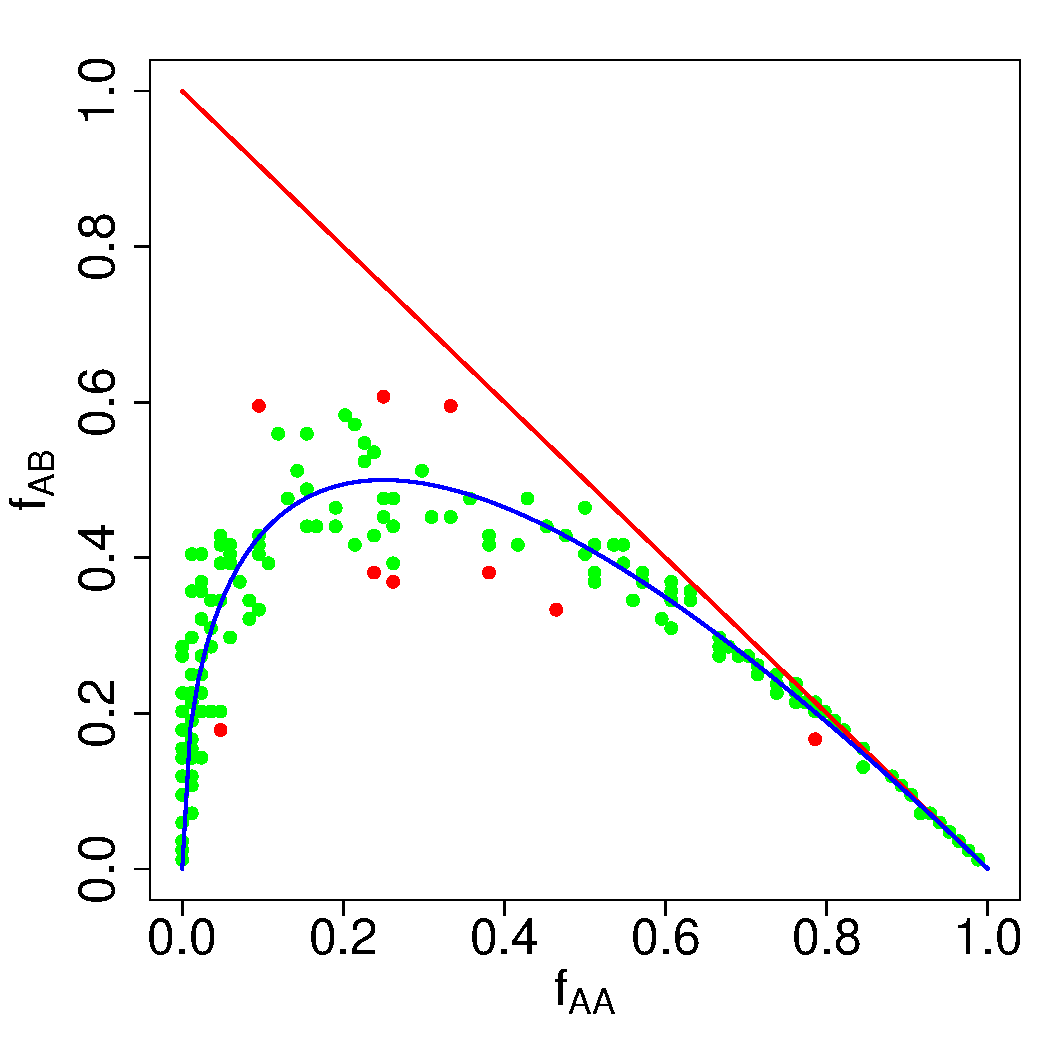
\includegraphics[width=.5\textwidth, trim=0 10 0 20, clip]{HWHapMapGeno1.pdf}%
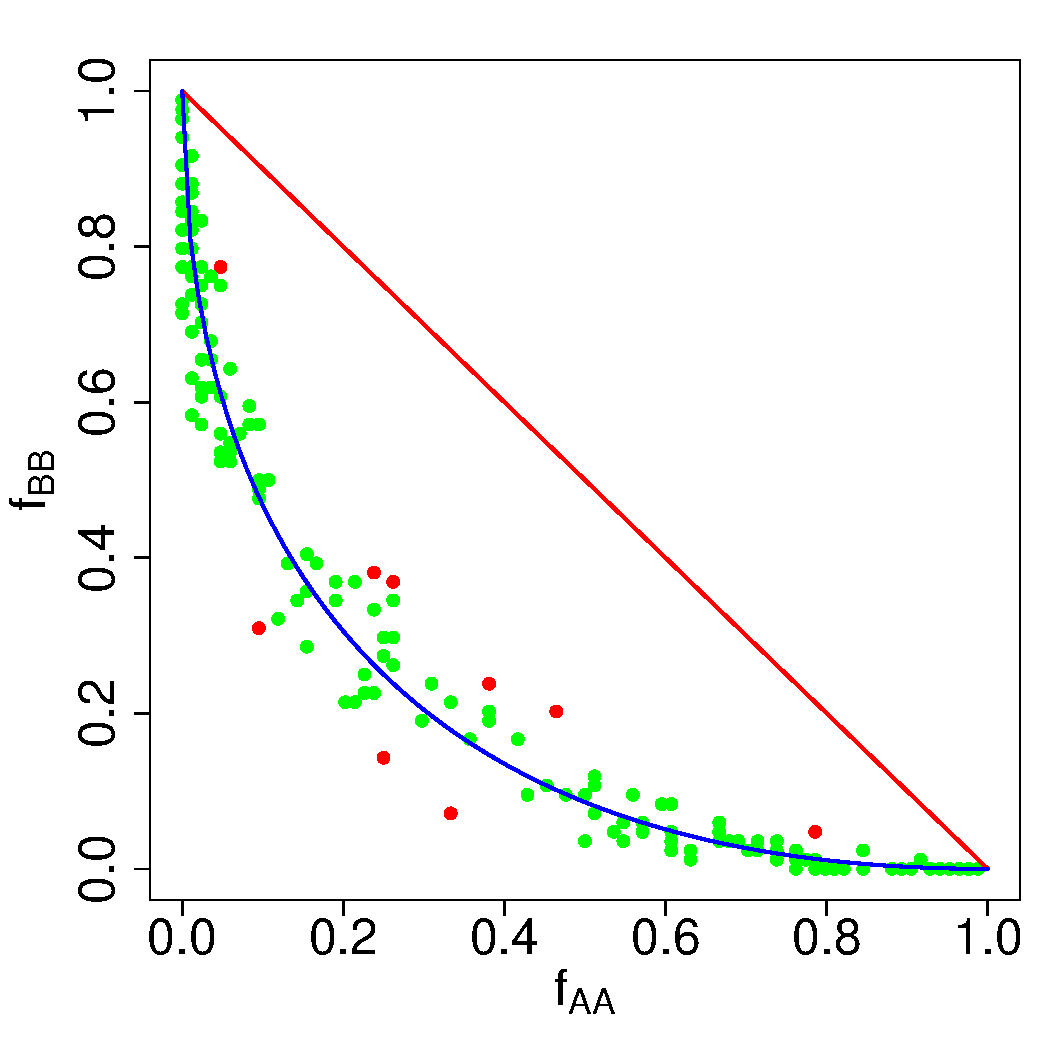
\includegraphics[width=.5\textwidth, trim=0 10 0 20, clip]{HWHapMapGeno2.pdf}
\caption{Genotype frequency scatter plots and HWE for 225 SNPs on
  chromosome 1 of a Han Chinese population. Significant markers
  (according to a chi-square test) are indicated by red points,
  non-significant markers by green points.  The blue curves in the
  plots indicate perfect HWE.}\label{fig:homhet}
\end{figure}

\subsection{The ternary plot}
\label{subsec:ternary}
The Italian statistician Bruno \cite{deFinetti}
represented genotype frequencies in a ternary diagram. This diagram is
known as a {\it de Finetti diagram} in the genetics
literature~\citep{Cannings}.  The HWE condition defines a parabola in
the ternary plot.  A ternary plot of the genotype frequencies with the
HWE parabola is an information-rich graphical display. From this plot
one can recover genotype frequencies, allele frequencies, and infer
the equilibrium status of a genetic marker at a glance (see
Figure~\ref{fig:ternary}).

\begin{figure}[t!]
\centering
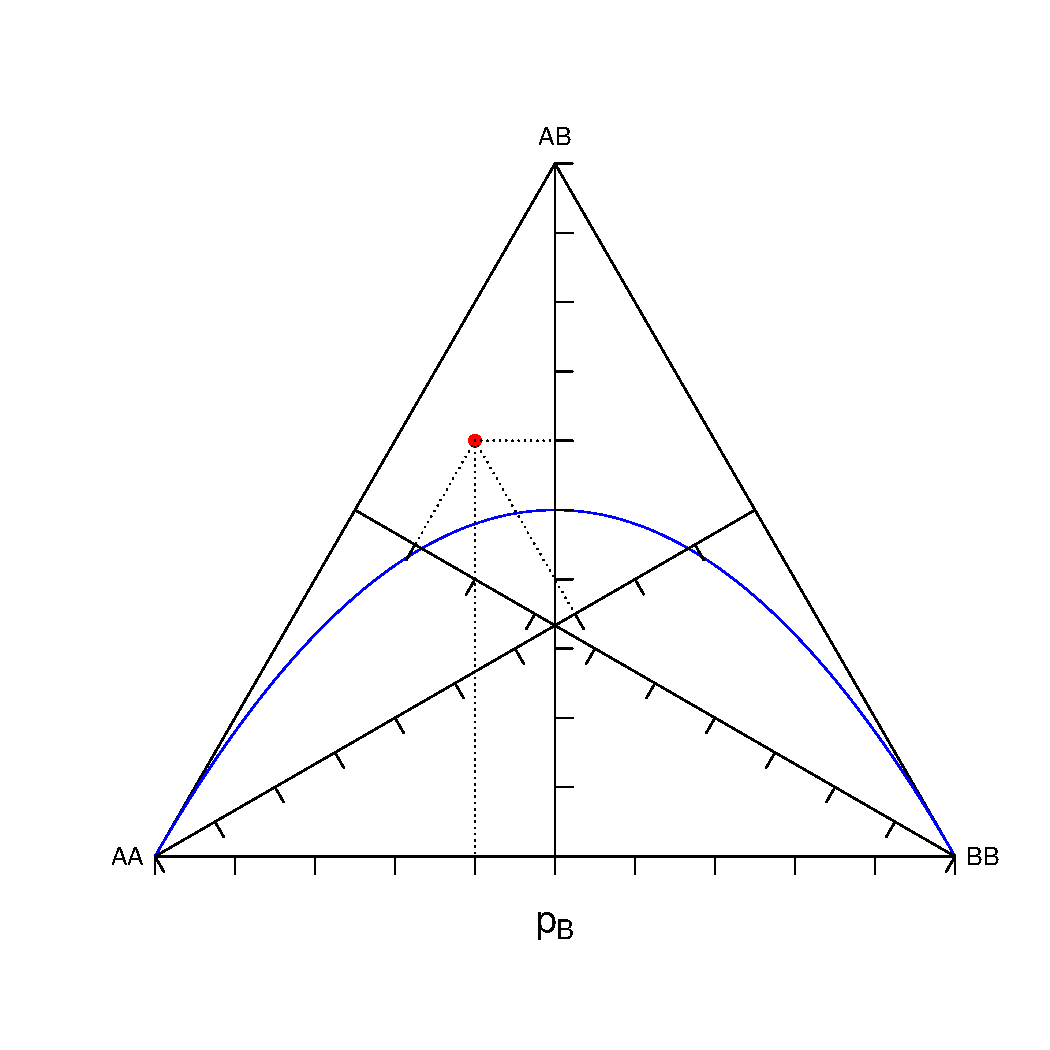
\includegraphics[width=.6\textwidth, trim=0 40 0 40, clip]{TernaryPlot.pdf}
\caption{Ternary plot of a genetic marker, showing the recovery of genotype frequencies ($\faa = 0.30, \fab = 0.60$ and
  $\fbb = 0.10$) and allele frequencies ($p_B = 0.40$). The parabola represents Hardy-Weinberg equilibrium.}
\label{fig:ternary}
\end{figure}
The ternary plot is most useful for plotting data consisting of
multiple samples that have all been genotyped for the same genetic
marker. In that case the three vertices of the display are fully
identified. An example is shown in Figure~\ref{fig:mourant} where the
genotype counts for the {\sc mn} blood group locus are shown for 216
samples of various human populations from different geographical
origin~\cite[Table 2.5]{Mourant}.
\begin{figure}[t!]
\centering
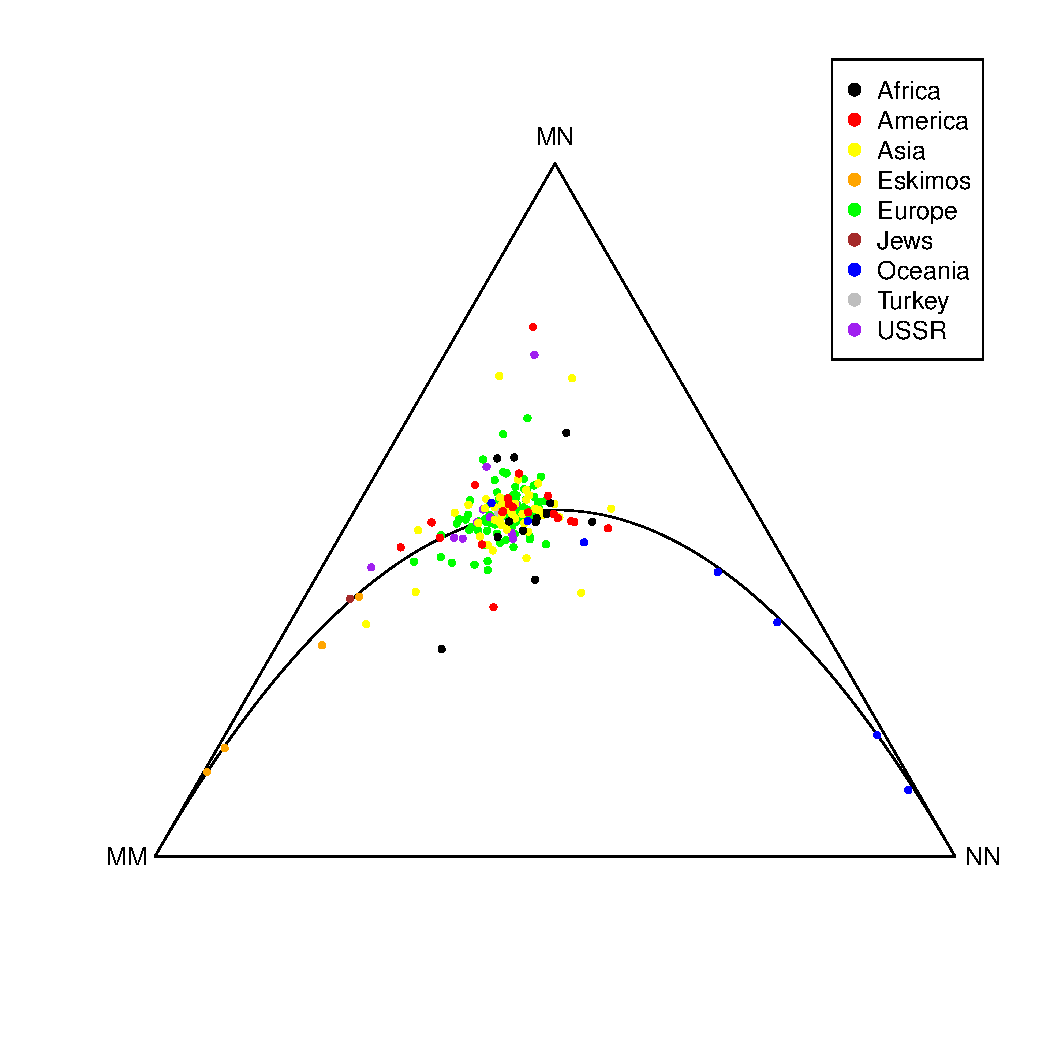
\includegraphics[width=0.5\textwidth, trim=0 60 0 20, clip]{MourantTP.pdf}%
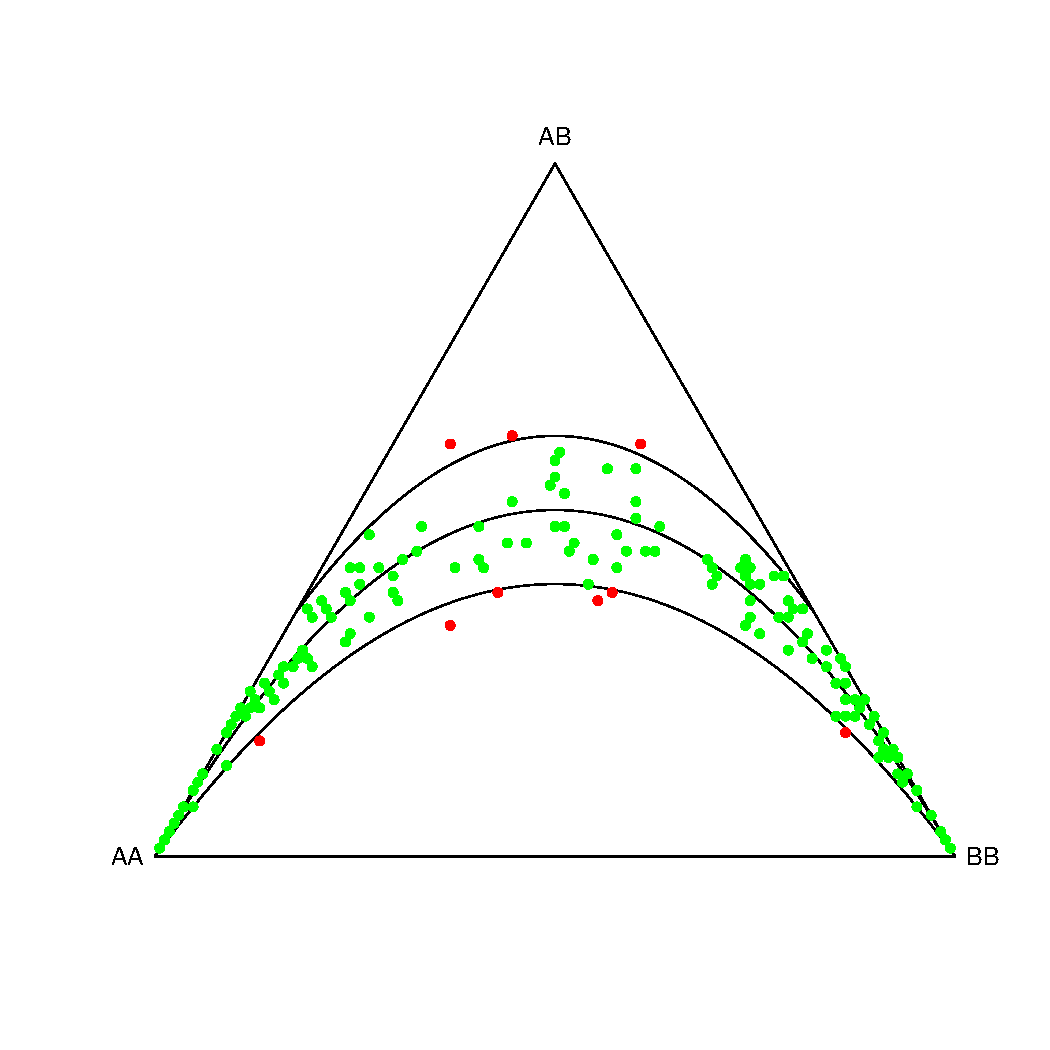
\includegraphics[width=0.5\textwidth, trim=0 60 0 20, clip]{HapMapCHBChr1.pdf}
\caption{Left panel: ternary plot for one marker: {\sc mn} blood group
  genotype frequencies for 216 samples from different human
  populations. Right panel: ternary plot for multiple markers: 225
  SNPs on chromosome 1 of a sample of 84 individuals from the Han
  Chinese population. HWE parabola and acceptance region for a
  chi-square test are shown in the latter plot.}\label{fig:mourant}
\end{figure}
The plot shows relatively higher allele frequencies for the {\sc n}
allele for samples from Oceania, and lower allele frequencies for this
allele for the Eskimo samples. African, American, European and Asian
populations have intermediate allele frequencies. Most samples clearly
cluster around the HWE parabola, though there are
several deviating samples as well.

The ternary plot may also be used to represent multiple markers,
though this is a bit tricky because the obtained display is no longer
uniquely determined. In this case, one vertex, usually the top vertex,
is chosen to represent the heterozygote frequency of each marker. The
two bottom vertices are used for one of the two homozygote
frequencies. It is arbitrary to place {\sc aa} on the right and {\sc
  bb} on the left or the other way round. Representing multiple
markers amounts to overplotting all ternary diagrams for each
individual marker in such a way that the axes for the heterozygotes
always coincide. Despite the indeterminacy of the homozygote vertices,
the plot remains highly informative, as now minor allele frequency,
genotype frequencies and equilibrium status are visualized
simultaneously for many markers in just one plot. \cite{Graffel18}
amplified the ternary plot by representing the acceptance regions of
chi-square and exact tests inside the plot. An example with multiple
markers is shown in the right panel of Figure~\ref{fig:mourant}. This
figure shows 225 SNPs of the dataset \code{HapMapCHBChr1}.  The
function \code{HWTernaryPlot} of the package allows the construction
of ternary plots with the equilibrium parabola and various acceptance
regions.  

\subsection{Log-ratio plots}
\label{subsec:log-ratio}
A vector of genotype counts ({\sc aa, ab, bb}) can be seen as a
composition, where these counts form parts of a whole. Compositional
data analysis~\citep{Aitchison} is a branch of statistics dedicated to
the analysis of compositions. Some of the tools employed in
compositional data analysis such as ternary diagrams and log-ratio
transformations can be useful for the analysis of genotype
counts. Currently, three types of log-ratio transformations are in use:
the additive log-ratio (alr) transformation, the centered log-ratio
(clr) transformation and the isometric log-ratio (ilr)
transformation~\citep{Egozcue2}. Starting with a vector of genotype
counts ($\bx = (\naa, \nab, \nbb)$), the log-ratio transformations for
diallelic markers were given by~\cite{Graffel21}, and are also
detailed below:
\begin{align}
\hspace{3mm} \alr(\mbf{x}) & = \left\{ \begin{array}{l}
              \left( \ln \frac{\faa}{\fab}, \ln \frac{\fbb}{\fab} \right),\\
              \left( \ln \frac{\fab}{\faa}, \ln \frac{\fbb}{\faa} \right),\\
              \left( \ln \frac{\faa}{\fbb}, \ln \frac{\fab}{\fbb} \right),\\
               \end{array} \label{eq:alr}
       \right. \\
\hspace{3mm} \clr(\mbf{x}) & = \left( \ln \frac{\faa}{\gm(\mbf{x})}, \ln \frac{\fab}{\gm(\mbf{x})}, \ln \frac{\fbb}{\gm(\mbf{x})} \right), \label{eq:clr}\\
\hspace{3mm} \ilr(\mbf{x}) & = \left\{ \begin{array}{l}
              \left( \frac{1}{\sqrt{2}} \ln  \frac{\faa}{\fbb}, \frac{1}{\sqrt{6}} \ln \frac{\faa \fbb}{\fab^2} \right),\\
              \left( \frac{1}{\sqrt{2}} \ln  \frac{\fab}{\fbb}, \frac{1}{\sqrt{6}} \ln \frac{\fab \fbb}{\faa^2} \right),\\
              \left( \frac{1}{\sqrt{2}} \ln  \frac{\faa}{\fab}, \frac{1}{\sqrt{6}} \ln \frac{\faa \fab}{\fbb^2} \right),\\
               \end{array} \label{eq:ilr}
       \right. 
\end{align}
where $\gm(\cdot)$ denotes the geometric mean of its argument. Note
that there exist 3 alr and 3 ilr transformations depending on which
genotype count is used as the divisor in the log-ratios. We will use
the first of the three ilr transformations, because the isometric
log-ratio transformation yields a space with an orthonormal basis, and
because HWE is in these coordinates represented by a simple horizontal
line. With this transformation, HWE implies that the second ilr
coordinate is constant ($-\sqrt{2/3} \lne{2}$) and the first
coordinate is $\sqrt{2}$ times the log odds of the allele frequency.
The package includes some standard routines for computing additive,
centered and isometric log-ratio coordinates for vectors of genotype
counts (\code{HWAlr, HWClr} and \code{HWIlr}), and also graphical
routines that display markers in log-ratio coordinates
(\code{HWAlrPlot, HWClrPlot} and \code{HWIlrPlot}).  HWE is
represented in log-ratio coordinates by a perfect linear relationship
between the first and second log-ratio coordinate. Examples of the
log-ratio plots for the Mourant data and the HapMap data are given in
Figure~\ref{fig:logratio}.

\begin{figure}[t!]
\centering
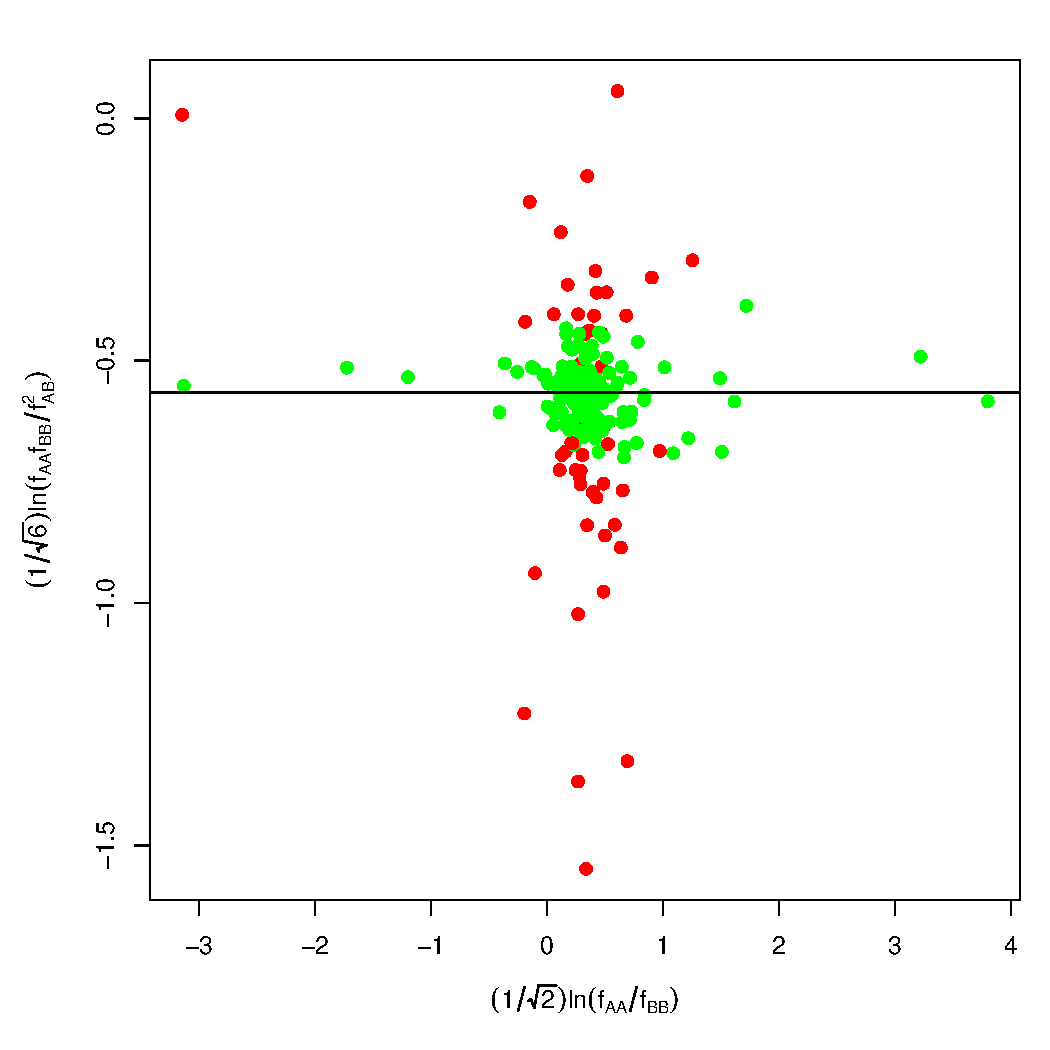
\includegraphics[width=0.5\textwidth, trim=0 10 0 20, clip]{HWHapMapIlr1.pdf}%
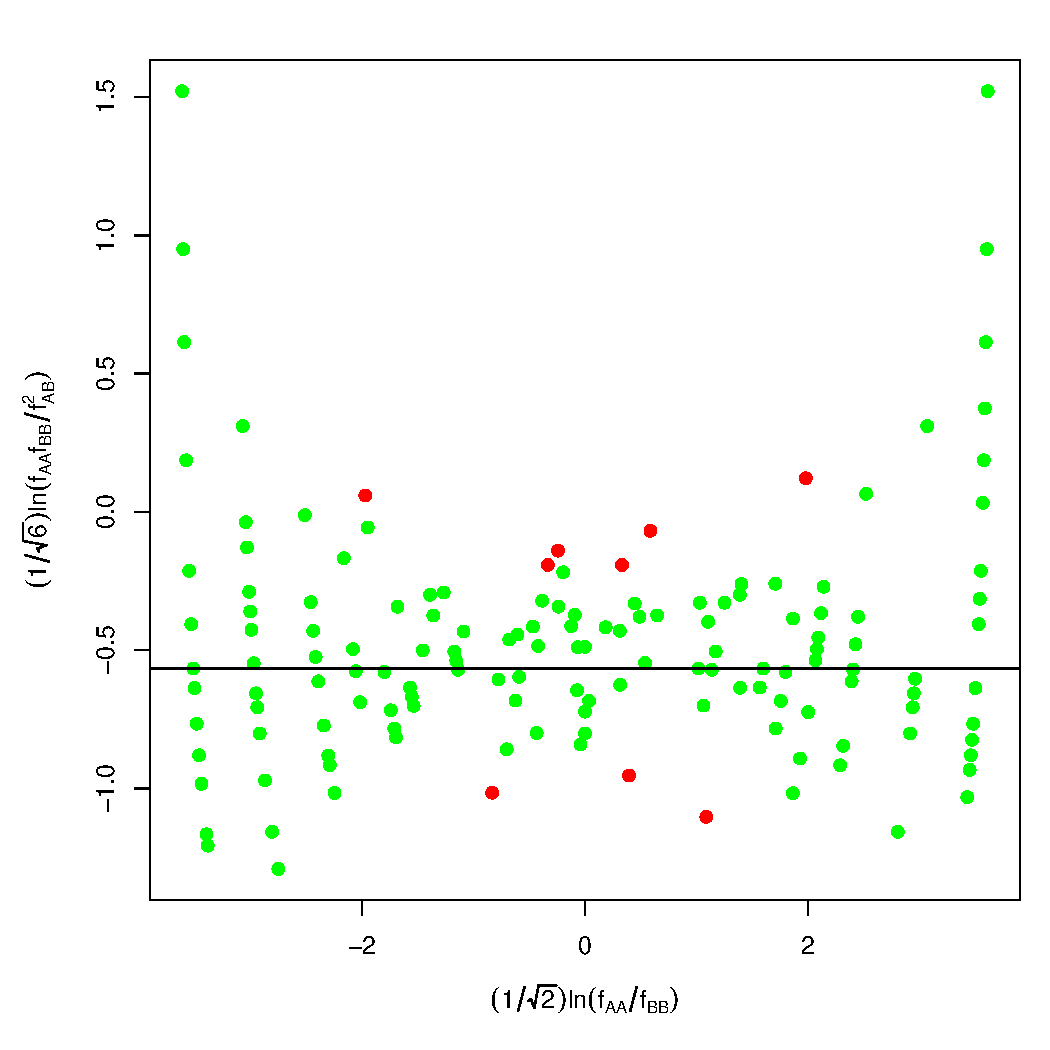
\includegraphics[width=0.5\textwidth, trim=0 10 0 20, clip]{HWHapMapIlr2.pdf}
\caption{Left panel: ilr plot of {\sc mn} blood group genotype
  frequencies for 216 samples from different human populations. Right
  panel: ilr plot for 225 SNPs on chromosome 1 of a sample of 84
  individuals from a Han Chinese population. HWE is represented by the
  horizontal line with ordinate $-\sqrt{2/3}\lne{2} = -0.57$. Markers
  are colored according to a chi-square test for HWE (red points
  significant, green points not significant).}\label{fig:logratio}
\end{figure}

\begin{figure}[t!]
\centering
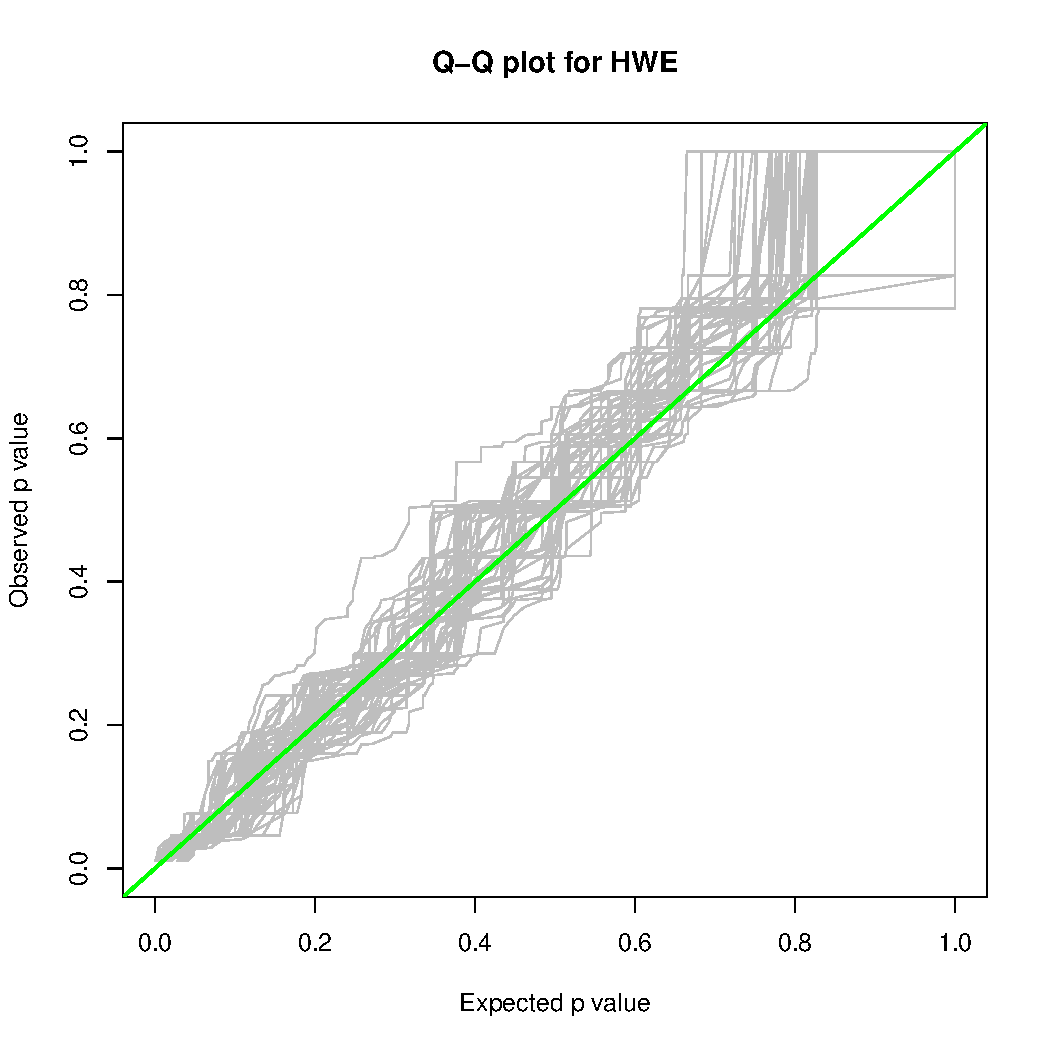
\includegraphics[width=0.5\textwidth, trim=0 10 0 20, clip]{HWHapMapQQplot.pdf}%
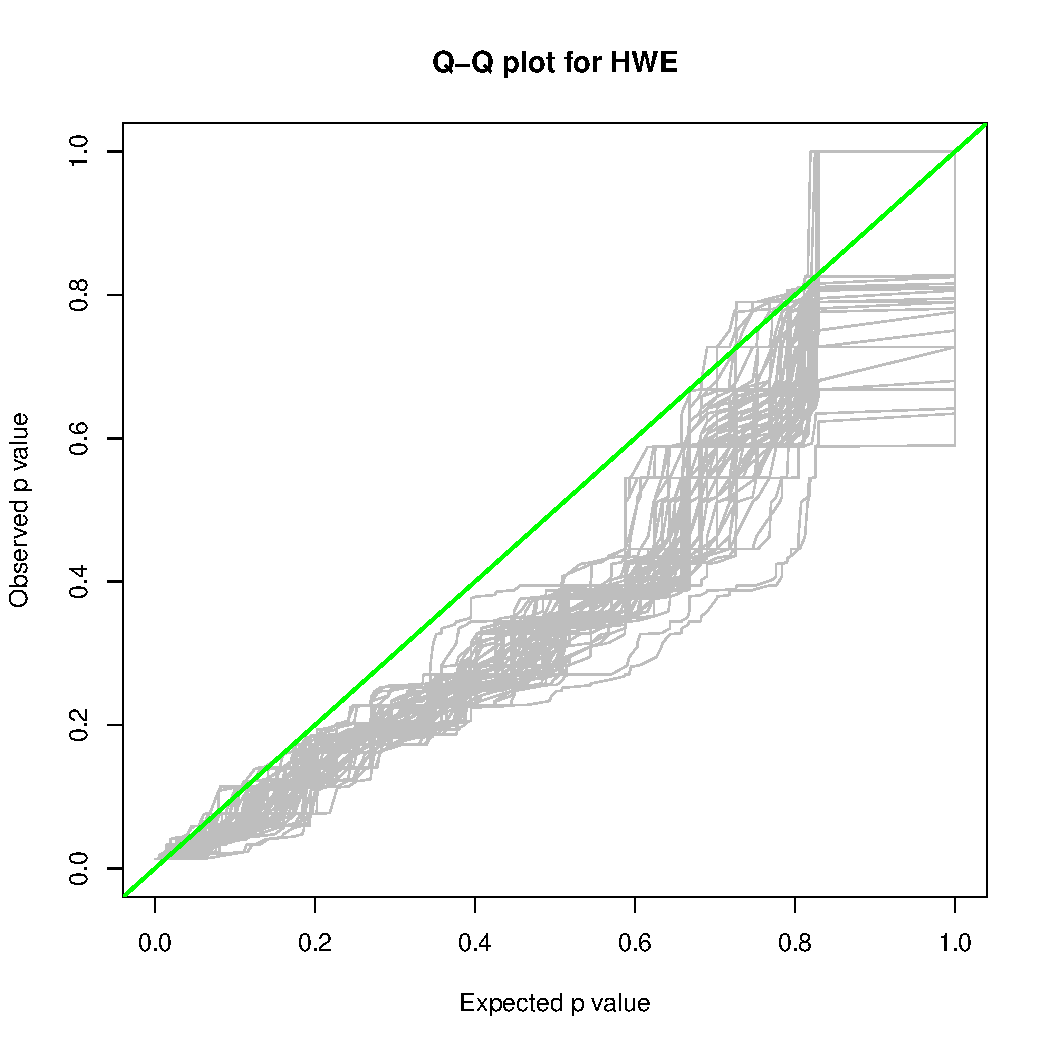
\includegraphics[width=0.5\textwidth, trim=0 10 0 20, clip]{HWHapMapQQplotInbred.pdf}
\caption{Left panel: Q-Q plot for 225 SNPs on chromosome 1 of a sample
  of 84 individuals from the Han Chinese population. Right panel: Q-Q
  plot for simulated data (225 SNPs, 84 individuals) with inbreeding
  ($f=0.05$).}\label{fig:qqplot}
\end{figure}

\subsection{Q-Q plots}
\label{subsec:q-q}
Genetic association studies nowadays investigate many markers for
their possible relation with diseases. The equilibrium status of the
markers is important, since deviation from HWE may be indicative of
genotyping error. Moreover, disequilibrium for cases in a case-control
study is indicative for disease association. Given that so many
markers are tested, it is cumbersome to do this all in a numerical
manner only, and it is known beforehand that false positives will
arise. Even if we find that 5\% of the markers is significant when we
use a significance level of $\alpha = 0.05$, this does not imply that
the database as a whole can be considered to be ``in
equilibrium''. The distribution of the test results (chi-square
statistics or $p$~values) then becomes interesting to look at. One way
to do this is to compare the sample percentiles of the chi-square
statistics of all markers with the theoretical percentiles of a
$\chi^2_1$ distribution in a chi-square quantile-quantile plot (Q-Q
plot). For exact tests, Q-Q plots of the $p$~values are used.
Often the uniform distribution is chosen as the reference
distribution. However, with discrete data the $p$~value distribution
under the null is not uniform. The function \code{HWQqplot} of the
package plots the $p$~values against samples from the null distribution
rather than the uniform distribution. The function takes into account
that sample size and allele frequency can vary over
markers. Figure~\ref{fig:qqplot} shows Q-Q plots for the HapMap data
(left panel) and also for simulated data under moderate inbreeding
(right panel, $f=0.05$). The green line is the reference line passing
through the origin with slope 1. Each grey line plots a sample from
the null distribution against the empirical quantiles of the
$p$~values. Deviation of the green line from the grey zone is taken as
evidence that HWE is violated. The HapMap data set is seen to be in
good agreement with what is expected under the null. This is not
surprising, as the markers of the project undergo a quality control
filter, and markers that strongly deviate from HWE ($p$~value of an exact
test < 0.001) are discarded from the project. For the dataset
simulated under inbreeding, a manifest deviation from HWE is
found. Q-Q plots assume independent observations. We note that this
assumption will be violated if the markers under study are closely
neighboring markers from the same region of a single chromosome.


\section{An example session}
\label{sec:session}

This section shows the basic use of the package for testing and
plotting genetic markers. We consider installation
(Section~\ref{subsec:install}), testing of markers
(Section~\ref{subsec:testing}), power computations
(Section~\ref{subsec:powercomp}), simulation of marker data
(Section~\ref{subsec:simulation}) and graphics for HWE
(Section~\ref{subsec:graphics}).

\subsection{Installation}
\label{subsec:install}

The \pkg{HardyWeinberg} package can be installed as usual via the command line or graphical
user interfaces, e.g., the package can be installed and loaded by:


\begin{Schunk}
\begin{Sinput}
R> install.packages("HardyWeinberg")
R> library("HardyWeinberg")
\end{Sinput}
\end{Schunk}

%
This will make, among others, the functions \code{HWChisq},
\code{HWData}, \code{HWExact}, \code{HWLratio}, \code{HWMissing},
\code{HWPower}, \code{HWQqplot}, and \code{HWTernaryPlot}
available. The document describing the package (this paper) can be
consulted from inside \proglang{R} by typing:
%

\begin{Schunk}
\begin{Sinput}
R> vignette("HardyWeinberg")
\end{Sinput}
\end{Schunk}


\subsection{Testing autosomal markers for HWE}
\label{subsec:testing}

We show how to perform several classical tests for Hardy-Weinberg
equilibrium. As an example we use a sample of 1000 individuals
genotyped for the {\sc mn} blood group locus described by
\citet[Table~2.4]{Hedrick}. We store the genotype counts (298, 489 and
213 for {\sc mm, mn} and {\sc nn} respectively) in a vector \code{x}:
%

\begin{Schunk}
\begin{Sinput}
R> library("HardyWeinberg")
R> x <- c(MM = 298, MN = 489, NN = 213)
R> HW.test <- HWChisq(x, verbose = TRUE)
\end{Sinput}
\begin{Soutput}
Chi-square test with continuity correction for Hardy-Weinberg equilibrium (autosomal)
Chi2 =  0.1789563 DF =  1 p-value =  0.6722717 D =  -3.69375 f =  0.01488253 
\end{Soutput}
\end{Schunk}

%
This shows that the chi-square statistic has value 0.179, and that the corresponding 
$p$~value for 
the test is 0.6723. Taking 
Taking a significance
level of $\alpha = 0.05$, we do not reject HWE for the {\sc mn}
locus. When \code{verbose} is set to \code{FALSE} (default) the test
is silent, and \code{HW.test} is a list object containing the results
of the test (chi-square statistic, the $p$~value of the test, half the
deviation from HWE (\code{D}) for the heterozygote ($D = \frac{1}{2}
(f_{AB} - e_{AB}$)), the minor allele frequency (\code{p}) and the
inbreeding coefficient \code{f}).  By default, \code{HWChisq} applies
a continuity correction. This is not recommended for low minor allele
frequencies. In order to perform a chi-square test without Yates'
continuity correction, it is necessary to set the \code{cc} parameter
to zero:
%

\begin{Schunk}
\begin{Sinput}
R> HW.test <- HWChisq(x, cc = 0, verbose = TRUE)
\end{Sinput}
\begin{Soutput}
Chi-square test for Hardy-Weinberg equilibrium (autosomal)
Chi2 =  0.2214896 DF =  1 p-value =  0.6379073 D =  -3.69375 f =  0.01488253 
\end{Soutput}
\end{Schunk}

%
The test with correction gives a smaller $\chi^2$-statistic and a
larger $p$~value in comparison with the ordinary $\chi^2$ test. The
likelihood ratio test for HWE can be performed by typing

\begin{Schunk}
\begin{Sinput}
R> HW.lrtest <- HWLratio(x, verbose = TRUE)
\end{Sinput}
\begin{Soutput}
Likelihood ratio test for Hardy-Weinberg equilibrium
G2 = 0.2214663 DF = 1 p-value = 0.637925 
\end{Soutput}
\end{Schunk}

%
%
Note that the $G^2$-statistic and the $p$~value obtained are very close to the chi-square statistic
and its $p$~value. An exact test for HWE can be performed by using routine \code{HWExact}. 
%
\begin{Schunk}
\begin{Sinput}
R> HW.exacttest <- HWExact(x, verbose = TRUE)
\end{Sinput}
\begin{Soutput}
Haldane Exact test for Hardy-Weinberg equilibrium (autosomal)
using SELOME p-value
sample counts: nMM =  298 nMN =  489 nNN =  213 
H0: HWE (D==0), H1: D <> 0 
D =  -3.69375 p-value =  0.6556635 
\end{Soutput}
\end{Schunk}
%

The exact test leads to the same conclusion, we do not reject HWE
($p$~value = 0.6557). Both one-sided and two-sided exact tests are
possible by using the argument \code{alternative}, which can be set to
\code{"two.sided"}, \code{"greater"}, or \code{"less"}. Three different ways
of computing the $p$~value of an exact test are implemented, and can be
specified by the \code{pvaluetype} argument, which can be set to
\code{dost} (double one-sided tail probability), \code{selome} (sum
equally likely or more extreme) or \code{midp} (the \midp\ $p$~value). The
exact test is based on a recursive algorithm. For very large samples,
\proglang{R} may give an error message "evaluation nested too deeply:
infinite recursion". This can usually be resolved by increasing
\proglang{R}'s limit on the number of nested expressions with
\code{options(expressions = 10000)} prior to calling \code{HWExact}. See
\code{?HWExact} for more information on this issue. The permutation test for HWE is activated by:

\begin{Schunk}
\begin{Sinput}
R> set.seed(123)
R> HW.permutationtest <- HWPerm(x, verbose = TRUE)
\end{Sinput}
\begin{Soutput}
Permutation test for Hardy-Weinberg equilibrium
Observed statistic: 0.2214896   17000 permutations. p-value: 0.6551765 
\end{Soutput}
\end{Schunk}

and the number of permutations can be specified via the \code{nperm} 
argument. By default the chi-square statistic will be used as the test statistic,
but alternative statistics may be supplied by the \code{FUN} argument.

All routines \code{HWChisq, HWExact, HWLratio} and \code{HWPerm} assume that
the data are supplied as a vector of genotype counts listed in order
({\sc aa, ab, bb}). The genotype counts may be specified in a
different other, but in that case the elements of the count vector
must be appropriately labeled. E.g., the \code{HWChisq} function may
also be called with:
%
\begin{Schunk}
\begin{Sinput}
R> x <- c(MN = 489, NN = 213, MM = 298)
R> HW.test <- HWChisq(x, verbose = TRUE)
\end{Sinput}
\begin{Soutput}
Chi-square test with continuity correction for Hardy-Weinberg equilibrium (autosomal)
Chi2 =  0.1789563 DF =  1 p-value =  0.6722717 D =  -3.69375 f =  0.01488253 
\end{Soutput}
\end{Schunk}

%
Often many markers are tested for HWE. If the genotype counts {\sc aa,
  ab, bb} are collected in a $m \times 3$ matrix, with each row
representing a marker, then HWE tests can be run over each row in the
matrix by the routines \code{HWChisqMat} and \code{HWExactMat}. These
routines return a list with the $p$~values and
test statistics for each marker.

If, for some reason, the equilibrium status of a particular marker is
at stake, you may wish to perform all tests to see to what extent they
do agree or disagree. You can use \code{HWAlltests} in order to
perform all tests with one call and obtain a table of all $p$~values.
%


\begin{Schunk}
\begin{Sinput}
R> HW.results <- HWAlltests(x, verbose = TRUE, include.permutation.test = TRUE)
\end{Sinput}
\begin{Soutput}
                                            Statistic   p-value
Chi-square test:                            0.2214896 0.6379073
Chi-square test with continuity correction: 0.1789563 0.6722717
Likelihood-ratio test:                      0.2214663 0.6379250
Exact test with selome p-value:                    NA 0.6556635
Exact test with dost p-value:                      NA 0.6723356
Exact test with mid p-value:                       NA 0.6330965
Permutation test:                           0.2214896 0.6422941
\end{Soutput}
\end{Schunk}

The {\sc mn} data concern a large sample ($n =$ 1000) with an intermediate allele frequency 
(p = 0.4575), for which all test results closely agree. For smaller samples
and more extreme allele frequencies, larger differences between the tests are typically observed.\\

We also indicate how to test for HWE when there is missing genotype
data. We use the data set \code{Markers} for that purpose.
%

\begin{Schunk}
\begin{Sinput}
R> data(Markers)
R> Markers[1:12,]
\end{Sinput}
\begin{Soutput}
   SNP1   iG   iT SNP2 SNP3
1    TT  641 1037   AA   GG
2    GT 1207  957   AC   AG
3    TT 1058 1686   AA   GG
4    GG 1348  466   CC   AA
5    GT 1176  948   AC   AG
6    GG 1906  912   CC   AA
7    GG 1844  705   CC   AA
8    GG 2007  599   CC   AA
9    GT 1369 1018   AC   AG
10   GG 1936  953   CC   AA
11   GG 1952  632   AC   AG
12 <NA>  947  920   AC   AG
\end{Soutput}
\end{Schunk}

%
Note that this data is at the level of each individual. Dataframe
\code{Markers} contains one SNP with missings (\code{SNP1}), the two
allele intensities of that SNP (\code{iG} and \code{iT}) and two
covariate markers (\code{SNP2} and \code{SNP3}). Here, the covariates
have no missing values. We first test \code{SNP1} for HWE using a
chi-square test and ignoring the missing genotypes:
% 


\begin{Schunk}
\begin{Sinput}
R> Xt <- table(Markers[,1])
R> Xv <- as.vector(Xt)
R> names(Xv) <- names(Xt)
R> HW.test <- HWChisq(Xv,cc=0,verbose=TRUE)
\end{Sinput}
\begin{Soutput}
Chi-square test for Hardy-Weinberg equilibrium (autosomal)
Chi2 =  8.67309 DF =  1 p-value =  0.003229431 D =  -6.77551 f =  0.297491 
\end{Soutput}
\end{Schunk}

%
This gives a significant result ($p$~value = 0.0032). 
If data can be
assumed to be missing completely at random (MCAR), then we may impute
missings by randomly sampling the observed data. This can be done by
supplying the \code{method = "sample"} argument, and we create 50
imputed data sets (\code{m = 50}).
%

\begin{Schunk}
\begin{Sinput}
R> set.seed(123)
R> Results <- HWMissing(Markers[,1], m = 50, method = "sample", verbose=TRUE)
\end{Sinput}
\begin{Soutput}
Test for Hardy-Weinberg equilibrium in the presence of missing values
Inbreeding coefficient f =  0.2936 
95 % Confidence interval ( 0.1058 , 0.4813 )
p-value =  0.0022 
Relative increase in variance of f due to missings: r =  0.3351 
Fraction of missing information about f: lambda =  0.2529 
\end{Soutput}
\end{Schunk}

%  
As could be expected, the conclusion is the same: there is significant
deviation from HWE ($p = $ 0.0022). It will make more sense to
take advantage of variables that are correlated with \code{SNP1}, and
use multiple imputation of the missings of \code{SNP1} using a
multinomial logit model. The multinomial logit model will be used when
we set \code{method = "polyreg"} or leave the \code{method} argument
out, since \code{"polyreg"} is the default for imputation of factor
variables by means of a multinomial logit model used by package
\pkg{mice}. We test \code{SNP1} (with missings) for HWE, using a
multinomial logit model to impute \code{SNP1} using information from
the allele intensities \code{iG} and \code{iT} and the neighboring
markers \code{SNP2} and \code{SNP3}.
%

\begin{Schunk}
\begin{Sinput}
R> set.seed(123)
R> Results <- HWMissing(Markers[, 1:5], m = 50, verbose = TRUE)
\end{Sinput}
\begin{Soutput}
Test for Hardy-Weinberg equilibrium in the presence of missing values
Inbreeding coefficient f =  0.0608 
95 % Confidence interval ( -0.1061 , 0.2278 )
p-value =  0.4751 
Relative increase in variance of f due to missings: r =  0.0596 
Fraction of missing information about f: lambda =  0.0564 
\end{Soutput}
\end{Schunk}

%
Note the sharp drop of the inbreeding coefficient, and the missing data statistics $\lambda$ and $r$. The test is now not 
significant ($p$~value = 0.4751). 
Exact inference for HWE with missings is possible
by setting the argument \code{statistic="exact"}. This gives the result

\begin{Schunk}
\begin{Sinput}
R> set.seed(123)
R> Results <- HWMissing(Markers[, 1:5], m = 50, statistic = "exact", verbose = TRUE)
\end{Sinput}
\begin{Soutput}
Two-sided Exact test for Hardy-Weinberg equilibrium in the presence of missing values
 p-value =  0.4426941 
\end{Soutput}
\end{Schunk}

and a similar $p$-value is obtained. See~\citet{Graffel24} for more details on
testing for HWE with missing data.

Autosomal tests for HWP assume equality of allele frequencies in the sexes. When sex is taken into account, several scenarios are possible. The function \code{HWPosterior} can be used to perform Bayesian model selection using the posterior probability of each scenario. We consider an example using an SNP of the JPT sample taken from the 1000G project.

\begin{Schunk}
\begin{Sinput}
R> data(JPTsnps)
R> Results <- HWPosterior(JPTsnps[1,],x.linked=FALSE,precision=0.05)
\end{Sinput}
\begin{Soutput}
  M_11   M_12   M_13   M_14   M_15   M_21   M_22   M_23   M_24   M_25 
0.6065 0.0061 0.0032 0.2595 0.0010 0.0675 0.0230 0.0246 0.0002 0.0084 
Best fitting M_11 0.606523 
\end{Soutput}
\end{Schunk}

The results show that for this variant, equality of allele frequencies in the sexes and HWP for both sexes (model $M_{11}$) is the model with the largest probability. For more accurate results, higher precision of posterior probabilities can be obtained by specifying {\tt precision=0.005}, at the expense of increasing the computation time.

We analyse the same variant by calculating the AIC for each scenario. This is achieved by

\begin{Schunk}
\begin{Sinput}
R> data(JPTsnps)
R> AICs <- HWAIC(JPTsnps[1,1:3],JPTsnps[1,4:6])
\end{Sinput}
\begin{Soutput}
Best fitting M_11 99.54001 
\end{Soutput}
\begin{Sinput}
R> AICs
\end{Sinput}
\begin{Soutput}
     M_11      M_12      M_13      M_14      M_15      M_21      M_22 
 99.54001 100.81297 100.55911  99.83219 101.83219 101.51680 102.78852 
     M_23      M_24      M_25 
102.53483 101.83219 103.80656 
\end{Soutput}
\end{Schunk}

In this case, the AIC criterion identifies the same $M_{11}$ model as the best fitting model.


\subsection{Testing X-chromosomal markers for HWE}
\label{subsec:testingx}

We show here how to perform HWE tests for X-chromosomal markers. We use a vector of 5
elements, containing male and female genotype counts.

\begin{Schunk}
\begin{Sinput}
R> SNP1 <- c(A=399,B=205,AA=230,AB=314,BB=107) 
R> HWChisq(SNP1,cc=0,x.linked=TRUE,verbose=TRUE)
\end{Sinput}
\begin{Soutput}
Chi-square test for Hardy-Weinberg equilibrium (X-chromosomal)
Chi2 =  7.624175 DF = 2 p-value =  0.022102 D =  NA f =  -0.0003817242 
\end{Soutput}
\end{Schunk}

When males are excluded from the test we get:

\begin{Schunk}
\begin{Sinput}
R> HWChisq(SNP1[3:5],cc=0)
\end{Sinput}
\begin{Soutput}
Chi-square test for Hardy-Weinberg equilibrium (autosomal)
Chi2 =  9.485941e-05 DF =  1 p-value =  0.9922291 D =  0.05990783 f =  -0.0003817242 
\end{Soutput}
\end{Schunk}

Note that the test including males is significant, whereas the test excluding males is not.

The exact test for HWE for an X-chromosomal marker can be performed by adding the \code{x.linked=TRUE} 
option:

\begin{Schunk}
\begin{Sinput}
R> HWExact(SNP1,x.linked=TRUE)
\end{Sinput}
\begin{Soutput}
Graffelman-Weir exact test for Hardy-Weinberg equilibrium on the X-chromosome
using SELOME p-value
Sample probability 5.682963e-05 p-value =  0.02085798 
\end{Soutput}
\end{Schunk}

which gives a $p$-value similar to the $\chi^2$ test. When the mid $p$-value is used we obtain

\begin{Schunk}
\begin{Sinput}
R> HWExact(SNP1,x.linked=TRUE,pvaluetype="midp")
\end{Sinput}
\begin{Soutput}
Graffelman-Weir exact test for Hardy-Weinberg equilibrium on the X-chromosome
using MID p-value
Sample probability 5.682963e-05 p-value =  0.02082957 
\end{Soutput}
\end{Schunk}

These exact tests show that the joint null of Hardy-Weinberg proportions \emph{and} equality of allele frequencies has to be rejected.
An exact test using the females only gives again a non-significant result:

\begin{Schunk}
\begin{Sinput}
R> HWExact(SNP1[3:5])
\end{Sinput}
\begin{Soutput}
Haldane Exact test for Hardy-Weinberg equilibrium (autosomal)
using SELOME p-value
sample counts: nAA =  230 nAB =  314 nBB =  107 
H0: HWE (D==0), H1: D <> 0 
D =  0.05990783 p-value =  1 
\end{Soutput}
\end{Schunk}

The permutation test for X-linked markers gives

\begin{Schunk}
\begin{Sinput}
R> HWPerm(SNP1,x.linked=TRUE)
\end{Sinput}
\begin{Soutput}
Permutation test for Hardy-Weinberg equilibrium of an X-linked marker
Observed statistic: 7.624175   17000 permutations. p-value: 0.02152941 
\end{Soutput}
\end{Schunk}

And an X-chromosomal likelihood ratio test givs

\begin{Schunk}
\begin{Sinput}
R> HWLratio(SNP1,x.linked=TRUE)
\end{Sinput}
\begin{Soutput}
Likelihood ratio test for Hardy-Weinberg equilibrium for an X-linked marker
G2 = 7.693436 DF = 2 p-value = 0.02134969 
\end{Soutput}
\end{Schunk}

Finally, a summary of all frequentist X-chromosomal tests is obtained by

\begin{Schunk}
\begin{Sinput}
R> HWAlltests(SNP1,x.linked=TRUE,include.permutation.test=TRUE)
\end{Sinput}
\begin{Soutput}
                                            Statistic    p-value
Chi-square test:                             7.624175 0.02210200
Chi-square test with continuity correction:  7.242011 0.02675576
Likelihood-ratio test:                       7.693436 0.02134969
Exact test with selome p-value:                    NA 0.02085798
Exact test with dost p-value:                      NA         NA
Exact test with mid p-value:                       NA 0.02082957
Permutation test:                            7.624175 0.02129412
\end{Soutput}
\end{Schunk}

Results of all tests are similar. Finally we test equality of allele frequencies in males and females with:

\begin{Schunk}
\begin{Sinput}
R> AFtest(SNP1)
\end{Sinput}
\begin{Soutput}
Fisher Exact test for equality of allele frequencies for males and females.

Table of allele counts:
    A   B
M 399 205
F 774 528

Sample of 1255 indivduals with 1906 alleles. p-value = 0.006268363
\end{Soutput}
\end{Schunk}

For this SNP, there is a significant difference in allele frequency 
between males and females. 

Puig, Ginebra and Graffelman~(\citeyear{Puig}) have proposed a Bayesian test for HWE for variants on the X-chromosome which is implemented in the function \code{HWPosterior}.

A Bayesian analysis of the same SNP is obtained by: 

\begin{Schunk}
\begin{Sinput}
R> HWPosterior(SNP1,x.linked=TRUE)
\end{Sinput}
\begin{Soutput}
Bayesian test for Hardy-Weinberg equilibrium of X-chromosomal variants.

                  Posterior_Prob log10(Bayes Factor)
M0 (HWE):                 0.3384              0.1859
M1 (f!=0):                0.0138             -1.3774
M2 (d!=1):                0.6222              0.6939
M3 (f!=0 & d!=1:)         0.0256             -1.1035
\end{Soutput}
\end{Schunk}

and shows that a model with Hardy-Weinberg proportions for females and different allele frequencies for both sexes has the 
largest posterior probability, and the largest Bayes factor.

\subsection{Testing  sets of markers for HWE}
\label{subsec:testingset}

Functions \code{HWCHisq, HWLratio, HWExact, HWPerm} test a single diallelic marker for HWE. 
Large sets of markers can be tested most efficiently with the functions \code{HWChisqStats} for the
chi-square test, and with \code{HWExactStats} for the exact tests. Both these functions allow for
X-linked markers via the \code{x.linked} argument. Exact tests that rely on exhaustive enumeration are slow in R, and \code{HWExactStats} now uses by default faster C++ code generously shared by Christopher Chang. The same C++ code is used in the current version (2.0) of Plink~(\cite{Purcell}).

\subsection{Power computation}
\label{subsec:powercomp}

Tests for HWE have low power for small samples with a low minor allele
frequency, or samples that deviate only moderately from HWE. It is
therefore important to be able to compute power. The function
\code{HWPower} can be used to compute the power of a test for HWE. If
its argument $\theta$ is set to 4 (the default value), then the
function computes the type I error rate for the test. Function
\code{mac} is used to compute the minor allele count. E.g.,:
%
\begin{Schunk}
\begin{Sinput}
R> x <- c(MM = 298, MN = 489, NN = 213)
R> n <- sum(x)
R> nM <- mac(x) 
R> pw4 <- HWPower(n, nM, alpha = 0.05, test = "exact", theta = 4, 
+                pvaluetype = "selome")
R> print(pw4)
\end{Sinput}
\begin{Soutput}
[1] 0.04822774
\end{Soutput}
\begin{Sinput}
R> pw8 <- HWPower(n, nM, alpha = 0.05, test = "exact", theta = 8, 
+                pvaluetype = "selome")
R> print(pw8)
\end{Sinput}
\begin{Soutput}
[1] 0.9996853
\end{Soutput}
\end{Schunk}

%
These computations show that for a large sample like this one, the type I error rate (0.0482) is
very close to the nominal rate, 0.05, and that the standard exact test has good power (0.9997) for
detecting deviations as large $\theta=8$, which is a doubling of the number of heterozygotes with respect to HWE.
Type I error rate and power for the chi-square test
can be calculated by setting \code{test="chisq"}.
With the allele frequency of this sample (0.5425), $\theta=8$ amounts to an inbreeding 
coefficient of -0.1698.

\subsection{Simulating data}
\label{subsec:simulation}

\begin{figure}[p!]
\centering
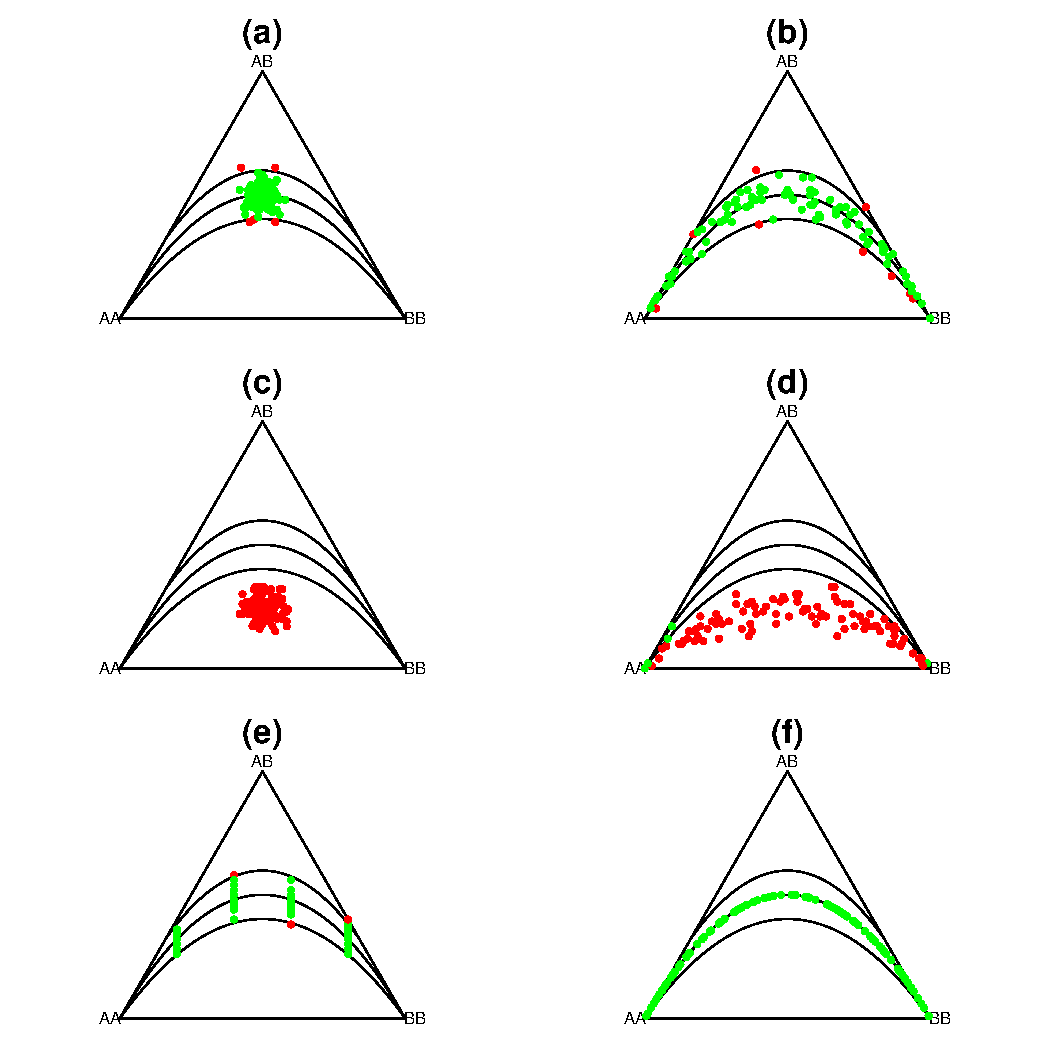
\includegraphics[width=\textwidth, trim=40 10 40 10, clip]{Simulated2.pdf} 
\caption{Ternary plots for markers simulated under different
  conditions. (a) multinomial sampling with $p=0.5$.  (b) multinomial
  sampling with a random uniform allele frequency. (c) multinomial
  sampling with $p=0.5$ and with inbreeding ($f=0.5$). (d) multinomial
  sampling with a random allele frequency with inbreeding ($f=0.5$).
  (e) sampling from the Levene-Haldane distribution with fixed allele
  frequencies. (f) a data set in exact equilibrium with a uniform
  allele frequency. Red points represent markers that are significant
  in a chi-square test for HWE, green points represent non-significant
  markers.}\label{fig:simulated}
\end{figure}

The package \pkg{HardyWeinberg} allows for the simulation of genetic
markers under equilibrium and disequilibrium conditions. This enables
the user to create simulated data sets that match the observed data
set in sample size and allele frequency. The comparison of graphics
and statistics for observed and simulated datasets is helpful when
assessing the extent of HWE for a large set of markers.  We simulate
$m=100$ markers for $n=100$ individuals by taking random samples from
a multinomial distribution with $\theta_{AA} = p^2, \hspace{1mm}
\theta_{AB} = 2pq, \hspace{1mm}$ and $\theta_{BB} = q^2$. This is done
by routine \code{HWData}, which can generate data sets that are in or
out of Hardy-Weinberg equilibrium. Routine \code{HWData} can generate
data that are in exact equilibrium (\code{exactequilibrium = TRUE}) or
that are generated from a multinomial distribution (default).  The
markers generated by \code{HWData} are independent (there is no
linkage disequilibrium).  \code{HWData} returns a list with both the
matrix of genotype counts \code{Xt} and the matrix with genotype
compositions \code{Xc} with the relative frequencies of {\sc aa, ab}
and {\sc bb}.  Routine \code{HWData} can simulate genotype counts
under several conditions. A fixed allele frequency can be specified by
setting \code{pfixed = TRUE}, and setting \code{p} to a vector with
the desired allele frequencies.  Sampling is then according to
Levene-Haldane's exact distribution in Equation~\ref{eq:exact}. If
\code{pfixed} is \code{FALSE}, the given vector \code{p} of allele
frequencies will be used in sampling from the multinomial
distribution. If \code{p} is not specified, \code{p} will be drawn
from a uniform distribution, and genotypes are drawn from a
multinomial distribution with probabilities $p^2, 2pq$ and $q^2$ for
{\sc aa}, {\sc ab} and {\sc bb} respectively. It is also possible to
generate data under inbreeding, by specifying a vector of inbreeding
coefficients \code{f}.  We illustrate the use of \code{HWData} by
simulating several data sets as shown below. Each simulated dataset is
plotted in a ternary diagram in Figure~\ref{fig:simulated2} in order to
show the effect of the different simulation options. We subsequently
simulate 100 markers under HWE with allele frequency 0.5 (\code{X1}),
100 markers under HWE with a random uniform allele frequency
(\code{X2}), 100 markers under inbreeding ($f = 0.5$) with allele
frequency 0.5 (\code{X3}), 100 markers under inbreeding ($f=0.5$) with
a random uniform allele frequency (\code{X4}), 100 markers with fixed
allele frequencies of 0.2, 0.4, 0.6 and 0.8 (25 each, \code{X5}) and
100 markers in exact equilibrium with a random uniform allele
frequency (\code{X6}).
%

\begin{Schunk}
\begin{Sinput}
R> set.seed(123)
R> n <- 100
R> m <- 100
R> X1 <- HWData(m, n, p = rep(0.5, m))
R> X2 <- HWData(m, n)
R> X3 <- HWData(m, n, p = rep(0.5, m), f = rep(0.5, m))
R> X4 <- HWData(m, n, f = rep(0.5, m))
R> X5 <- HWData(m, n, p = rep(c(0.2, 0.4, 0.6, 0.8), 25), pfixed = TRUE)
R> X6 <- HWData(m, n, exactequilibrium = TRUE)
R> opar <- par(mfrow = c(3, 2),mar = c(1, 0, 3, 0) + 0.1)
R> par(mfg = c(1, 1))
R> HWTernaryPlot(X1, main = "(a)", vbounds = FALSE)
R> par(mfg = c(1, 2))
R> HWTernaryPlot(X2, main = "(b)", vbounds = FALSE)
R> par(mfg = c(2, 1))
R> HWTernaryPlot(X3, main = "(c)", vbounds = FALSE)
R> par(mfg = c(2, 2))
R> HWTernaryPlot(X4, main = "(d)", vbounds = FALSE)
R> par(mfg = c(3, 1))
R> HWTernaryPlot(X5, main = "(e)", vbounds = FALSE)
R> par(mfg = c(3, 2))
R> HWTernaryPlot(X6, main = "(f)", vbounds = FALSE)
R> par(opar)
\end{Sinput}
\end{Schunk}

\begin{figure}
\begin{center}
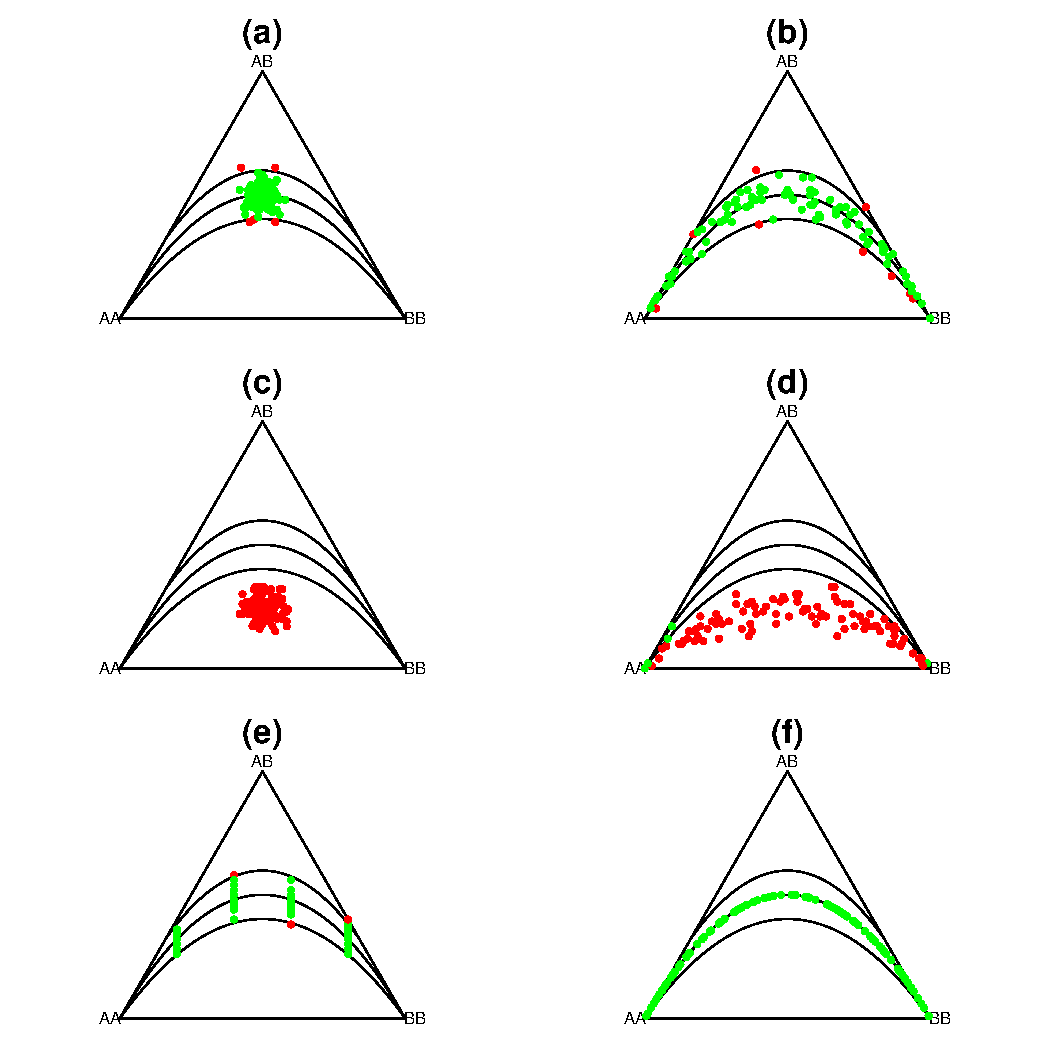
\includegraphics[height=120mm, width=120mm]{Simulated2.pdf} 
\caption{Ternary plots for markers simulated under different conditions. (a) multinomial sampling with $p=0.5$. 
  (b) multinomial sampling with a random uniform allele frequency. (c) multinomial sampling with $p=0.5$ and 
  with inbreeding ($f=0.5$). (d) multinomial sampling with a random allele frequency with inbreeding ($f=0.5$).
  (e) sampling from the Levene-Haldane distribution with fixed allele frequencies, (f) a data set in exact equilibrium with a uniform allele frequency. Red points represent markers that are significant in a chi-square test for HWE, green points represent non-significant markers.}\label{fig:simulated2}
\end{center}
\end{figure}
\clearpage


\subsection{Graphics for HWE}
\label{subsec:graphics}

Genetic association studies, genome-wide association studies in
particular, use many genetic markers. In this context graphics such as
ternary plots, log-ratio plots and Q-Q plots become particularly
useful, because they can reveal whether HWE is a reasonable assumption
for the whole data set. We begin to explore the Han Chinese HapMap
data set by making a ternary plot shown in Figure~\ref{fig:Han}.
%
\begin{Schunk}
\begin{Sinput}
R> data("HapMapCHBChr1", package = "HardyWeinberg")
R> HWTernaryPlot(HapMapCHBChr1, region = 1, vbounds = FALSE)
R> HWTernaryPlot(HapMapCHBChr1, region = 7, vbounds = FALSE)
\end{Sinput}
\end{Schunk}
%
\begin{figure}[b!]
\centering
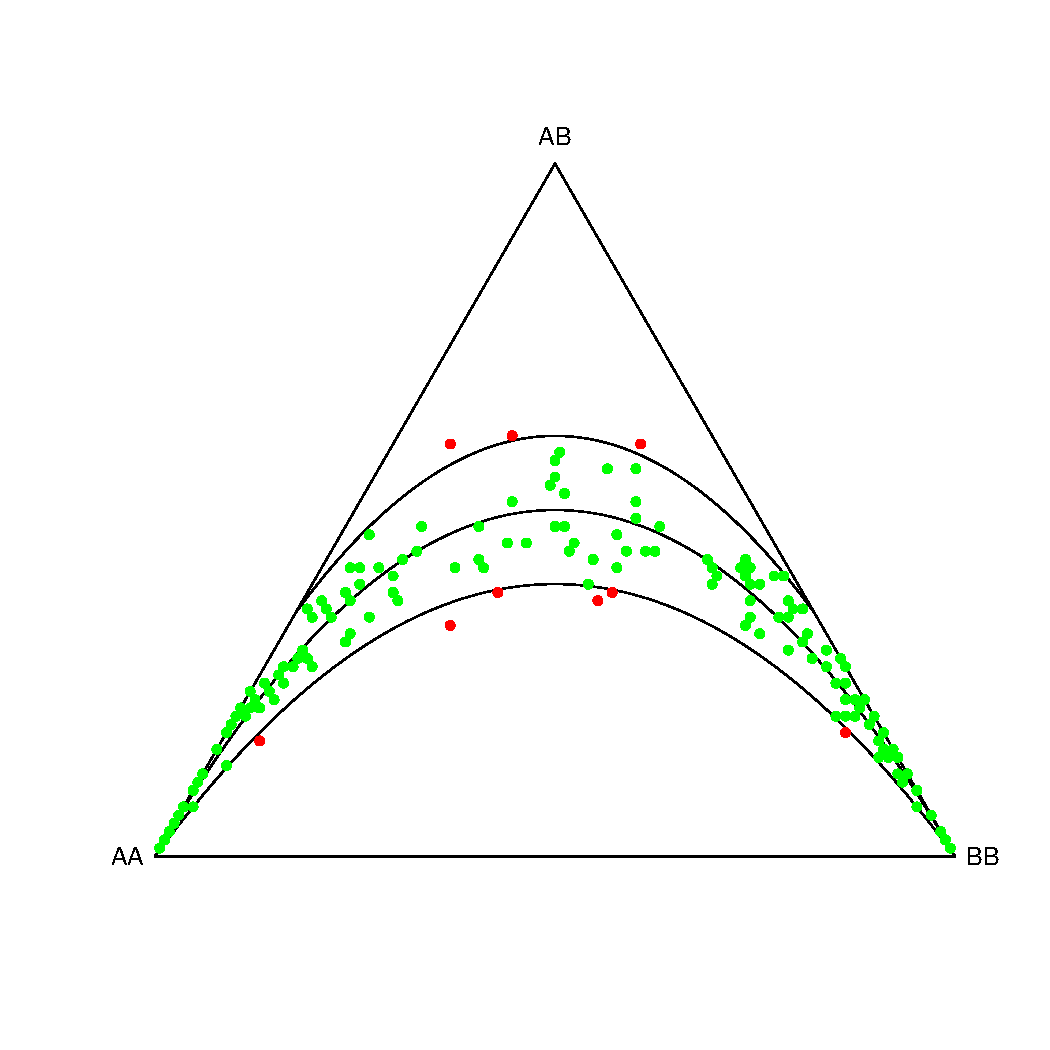
\includegraphics[width=0.5\textwidth, trim=40 70 20 40, clip]{HapMapCHBChr1Chisq.pdf}%
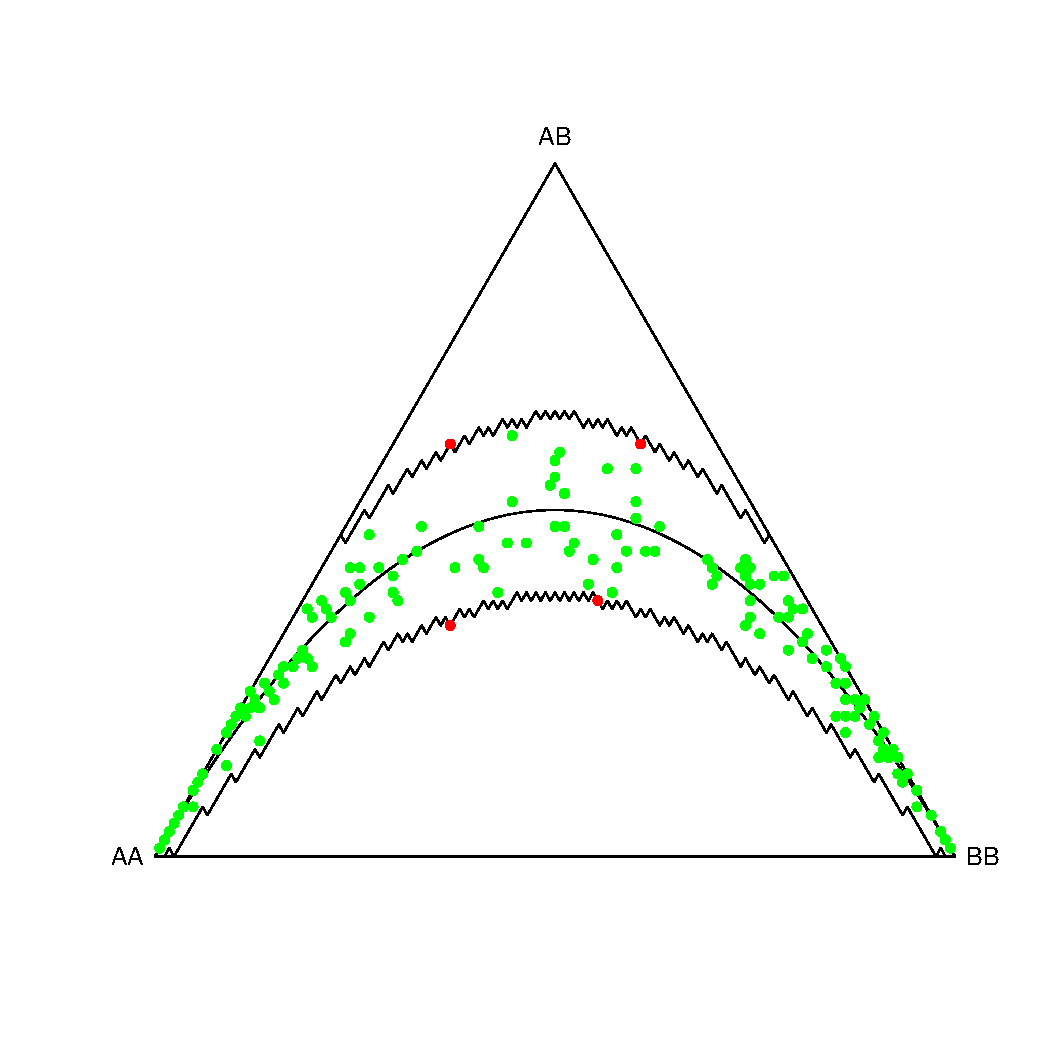
\includegraphics[width=0.5\textwidth, trim=20 70 20 40, clip]{HapMapCHBChr1Exact.pdf}
\caption{\label{fig:Han}Ternary plots of 225 SNPs on chromosome 1 of a
  sample of 84 individuals from a Han Chinese population. Left panel:
  ternary plot with the acceptance region of a chi-square test. Right
  panel: ternary plot with the acceptance region of an exact test.}
\end{figure}
%
For large databases of SNPs, drawing the ternary plot can be time
consuming. Usually the matrix with genotype counts contains several
rows with the same counts. The ternary plot can be constructed faster
by plotting only the unique rows of the count matrix. Function
\code{UniqueGenotypeCounts} extracts the unique rows of the count
matrix and also counts their frequency. Figure~\ref{fig:Han} shows 10
significant SNPs (two significant markers overlap). A ternary plot
with the acceptance region of the exact test is shown in the right
panel of Figure~\ref{fig:Han}. This plot only shows 4 significant
markers, and illustrates that the exact test is more conservative. A
log-ratio plot of the same data was already shown in
Figure~\ref{fig:logratio}, and can be created with
\code{HWIlrPlot(HapMapCHBChr1)}. We proceed to make a Q-Q plot of the
exact $p$~values. At the same time, we construct a simulated database
that matches the \code{HapMapCHBChr1} database in allele frequency
distribution. This is achieved by setting argument \code{p} of
\code{HWData} equal to the allele frequencies of the observed data,
where the latter are computed with function \code{af}.
%

\begin{Schunk}
\begin{Sinput}
R> set.seed(123)
R> data("HapMapCHBChr1", package = "HardyWeinberg")
R> HWQqplot(HapMapCHBChr1)
R> dev.off()
R> set.seed(123)
R> SimulatedData <- HWData(nm = 225, n = 84, p = af(HapMapCHBChr1))$Xt
R> HWQqplot(SimulatedData)
\end{Sinput}
\end{Schunk}

The Q-Q plots in Figure~\ref{fig:qqplot2} show that both the HapMap
dataset and its simulated counterpart are in agreement with HWE.

\begin{figure}[t!]
\centering
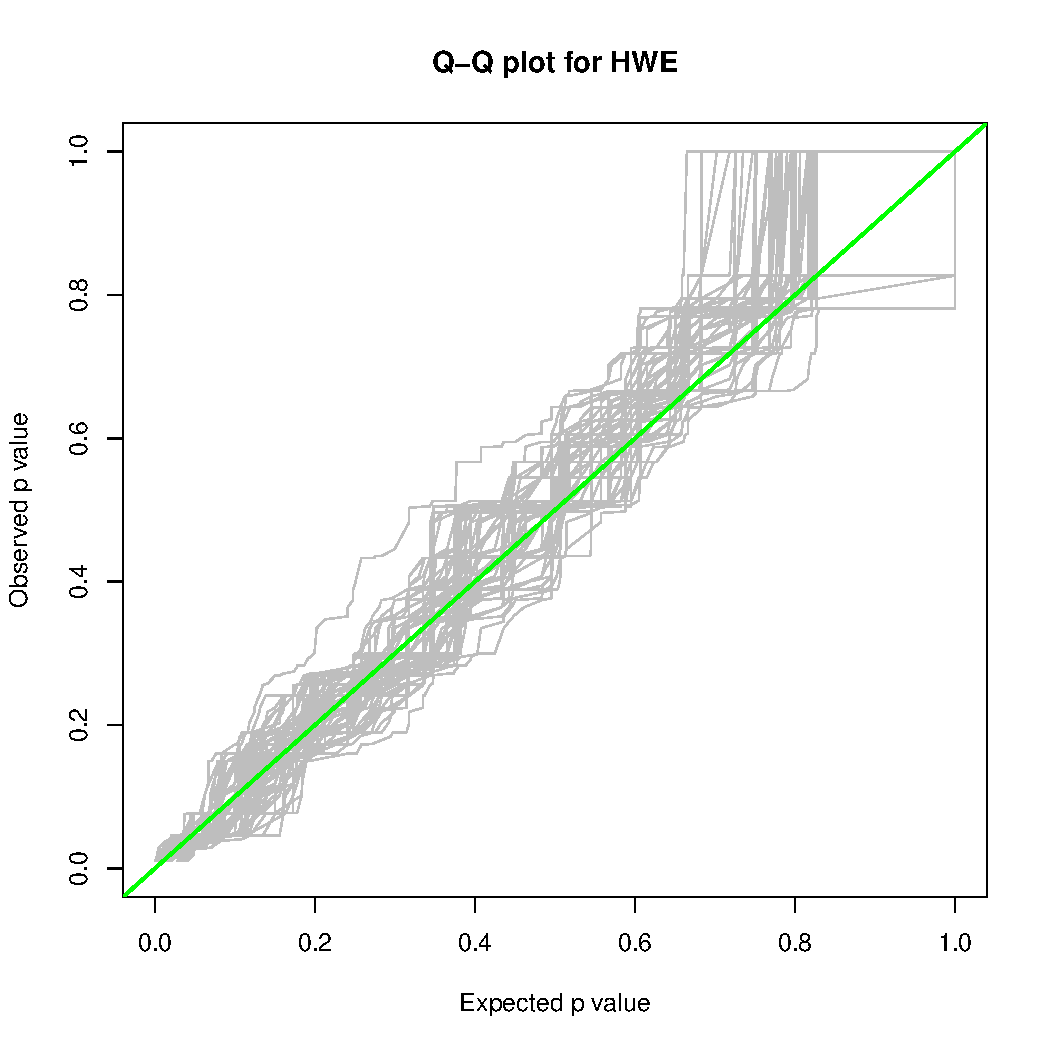
\includegraphics[width=.5\textwidth, trim=0 10 0 20, clip]{HWHapMapQQplot.pdf}%
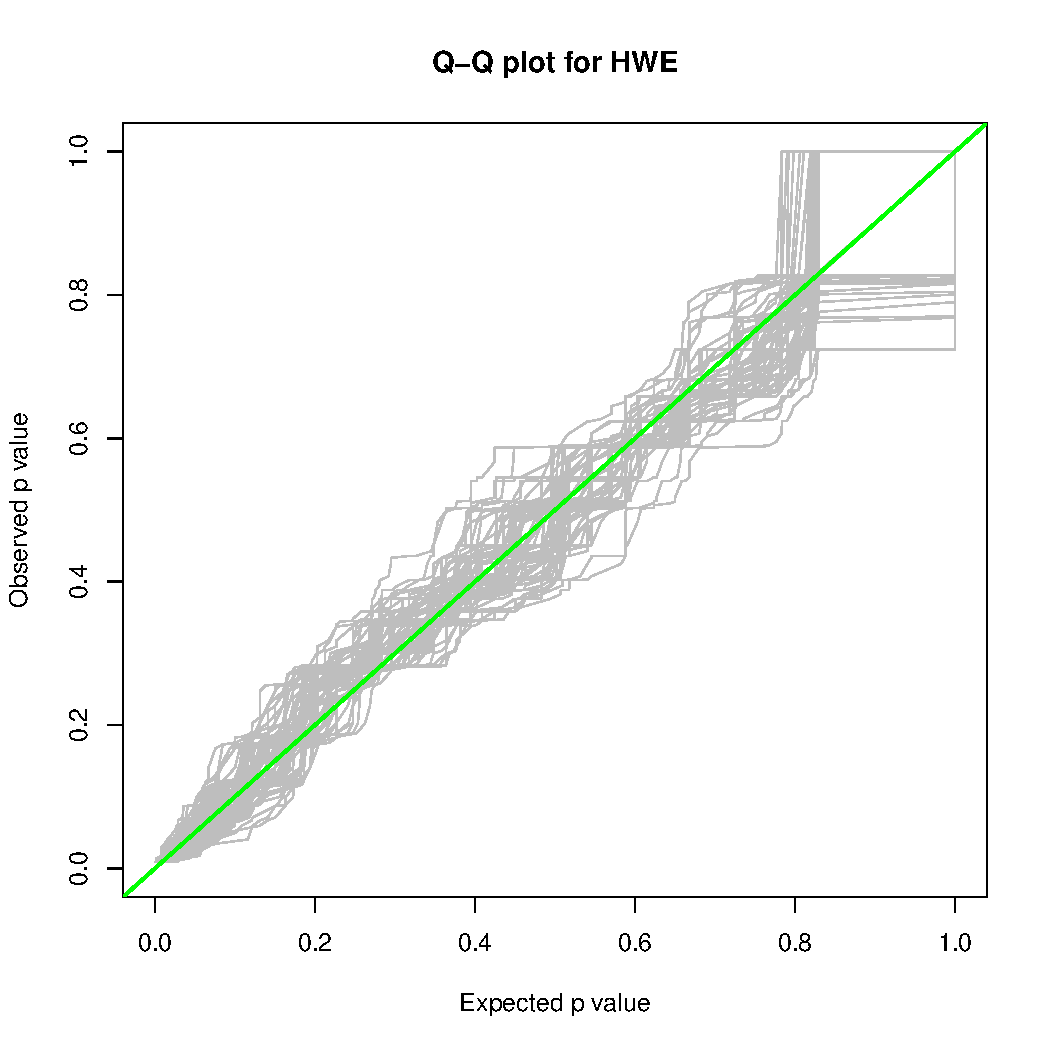
\includegraphics[width=.5\textwidth, trim=0 10 0 20, clip]{HWHapMapQQplotSimulated.pdf}
\caption{Left panel: Q-Q plot for 225 SNPs on chromosome 1 of a sample
  of 84 individuals from the Han Chinese population. Right panel: Q-Q
  plot for simulated data (225 SNPs, 84 individuals, matched in allele
  frequency).}\label{fig:qqplot2}
\end{figure}

\section{Discussion}
\label{sec:others}

The package \pkg{HardyWeinberg} offers functions
and graphics for analyzing the Hardy-Weinberg equilibrium status of
diallelic genetic markers. There are several other packages for the
\proglang{R} environment that implement functionality for
investigating genetic markers for HWE. The package \pkg{genetics}
by~\cite{Warnes} offers data structures for genetic markers, and also
includes several functions for testing markers for HWE and for linkage
equilibrium. Bayesian tests for HWE are implemented in the package
\pkg{HWEBayes} of~\cite{Wakefield} and the package \pkg{HWEintrinsic}
of~\cite{Venturini}. A loglinear modeling approach to HWE is available
in the package \pkg{hwde} from~\cite{Maindonald}.  The \pkg{PLINK}
software by \citet{Purcell} is a standard in
genetic data analysis, and can interact with \proglang{R} by means of
the package \pkg{Rserve} \citep{Rserve}.

We briefly enumerate and comment some features of the
\pkg{HardyWeinberg} package not provided by the aforementioned
\proglang{R} packages: the package provides several graphics for HWE
(ternary plots with acceptance regions, log-ratio plots and Q-Q plots
against the truly null distribution). These graphics are useful for
analyzing datasets of multiple markers (e.g., a set of markers used in
a candidate gene study, or the study of a specific genomic region),
and can shed light on the question if the HWE assumption is tenable
for the dataset as a whole. The functions provided for the simulation
of marker data under HWE (and under disequilibrium) are also useful in
this respect. They allow to create datasets that are similar to the
observed data in terms of sample size and allele frequency
distribution. The comparison of HWE graphics for simulated and
observed data can help to rule out or confirm the HWE
assumption. Functions for power calculation make it possible to
compute the power to detect deviation from HWE for the data at
hand. The exact tests of the package are apparently the only ones
available that implement several types of $p$~values, and
\pkg{HardyWeinberg} is apparently the only software package that performs
inference for HWE with missing genotype information using multiple
imputation. Future versions of the package may incorporate functions
for testing for HWE with multiple alleles. All tests of the package
assume homogeneous samples of individuals from one population. Testing
for HWE with individuals from different populations (stratification)
may also be addressed in future versions of the package.

\section*{Acknowledgments}

This work was partially supported by grant 2014SGR551 from the 
Ag\`encia de Gesti\'o d'Ajuts Universitaris i de Recerca (AGAUR) of the 
Generalitat de Catalunya and by grant MTM2012-33236 of the 
Spanish Ministry of Economy and Competitiveness.
This
document was generated using \code{Sweave}~\citep{Leisch}. I thank two anonymous
referees for their comments that have helped to improve the package
and the paper. I also thank professor Steve Marron from the University
of North Carolina for his comments on sampling fluctuations in Q-Q
plots.

\bibliography{HardyWeinberg}

\end{document}
